%!TEX TS-program = xelatex
%!TEX options = -aux-directory=Debug -shell-escape -file-line-error -interaction=nonstopmode -halt-on-error -synctex=1 "%DOC%"
\documentclass{article}
\input{LaTeX-Submodule/template.tex}

% Additional packages & macros
\usepackage{mathdots}

\DeclareMathOperator*{\argmax}{arg\,max}
\DeclareMathOperator*{\argmin}{arg\,min}
\DeclareMathOperator*{\nullity}{nullity}

% Header and footer
\newcommand{\unitName}{Advanced Linear Algebra}
\newcommand{\unitTime}{Semester 1, 2022}
\newcommand{\unitCoordinator}{Prof Timothy Moroney}
\newcommand{\documentAuthors}{\textsc{Tarang Janawalkar}}

\fancyhead[L]{\unitName}
\fancyhead[R]{\leftmark}
\fancyfoot[C]{\thepage}

% Copyright
\usepackage[
    type={CC},
    modifier={by-nc-sa},
    version={4.0},
    imagewidth={5em},
    hyphenation={raggedright}
]{doclicense}

\date{}

\begin{document}
%
\begin{titlepage}
    \vspace*{\fill}
    \begin{center}
        \LARGE{\textbf{\unitName}} \\[0.1in]
        \normalsize{\unitTime} \\[0.2in]
        \normalsize\textit{\unitCoordinator} \\[0.2in]
        \documentAuthors
    \end{center}
    \vspace*{\fill}
    \doclicenseThis
    \thispagestyle{empty}
\end{titlepage}
\newpage
%
\tableofcontents
\newpage
%
\section{Fundamental Concepts of Linear Algebra}
\subsection{Row Echelon Form}
We can solve linear systems by applying the following elementary row
operations to any matrix \(\symbf{A}\):
\begin{enumerate}[label=Type \Roman*.]
    \item Exchange any two rows.
    \item Multiply any row by a constant.
    \item Add a multiple of one row to another row.
\end{enumerate}
This allows us to reduce \(\symbf{A}\) into \textbf{row echelon form}
such that the entries below the main diagonal are zero:
\begin{equation*}
    \symbf{R}_{\mathrm{ref}} =
    \begin{bmatrix}
        r_{11} & r_{12} & \cdots & r_{1n} \\
               & r_{22} & \cdots & r_{2n} \\
               &        & \ddots & \vdots \\
               &        &        & r_{mn}
    \end{bmatrix}
\end{equation*}
\subsection{Elementary Matrix}
Mathematically, we can represent these row operations as a matrix which
is left multiplied to \(\symbf{A}\).
\begin{definition}[Elementary matrix]
    An elementary matrix \(\symbf{E}_i\) is constructed by applying a row operation to the elementary matrix \(\symbf{I}_m\).
    Consider a 3 by 4 matrix \(\symbf{A}\); a common first elementary row operation might be
    \begin{equation*}
        r_2 \leftarrow r_2 - \frac{a_{21}}{a_{11}} r_1
    \end{equation*}
    which when applied to \(\symbf{I}_3\), yields
    \begin{equation*}
        \symbf{E}_1 =
        \begin{bmatrix}
            1                      & 0 & 0 \\
            -\frac{a_{21}}{a_{11}} & 1 & 0 \\
            0                      & 0 & 1
        \end{bmatrix}
    \end{equation*}
    where the 1 subscript indicates the first of many elementary row operations.
    Left multiplying this to an arbitrary \(\symbf{A}\) gives
    \begin{align*}
        \symbf{E}_1 \symbf{A} & =
        \begin{bmatrix}
            1                      & 0 & 0 \\
            -\frac{a_{21}}{a_{11}} & 1 & 0 \\
            0                      & 0 & 1
        \end{bmatrix}
        \begin{bmatrix}
            a_{11} & a_{12} & a_{13} & a_{14} \\
            a_{21} & a_{22} & a_{23} & a_{24} \\
            a_{31} & a_{32} & a_{33} & a_{34}
        \end{bmatrix}
        \\
                              & =
        \begin{bmatrix}
            a_{11} & a_{12}                              & a_{13}                              & a_{14}                              \\
            0      & a_{22}-\frac{a_{12} a_{21}}{a_{11}} & a_{23}-\frac{a_{13} a_{21}}{a_{11}} & a_{24}-\frac{a_{14} a_{21}}{a_{11}} \\
            a_{31} & a_{32}                              & a_{33}                              & a_{34}
        \end{bmatrix}
    \end{align*}
    which has the desired result of eliminating the first column of the second row.
\end{definition}
\subsection{Reduced Row Echelon Form}
As there are infinitely many ways to reduce a matrix to row echelon
form, we typically reduce \(\symbf{R}_{\mathrm{ref}}\) further into
\textbf{reduced row echelon form} which is a unique reduction for all
matrices \(\symbf{A}\). This matrix \(\symbf{R}_{\mathrm{rref}}\) (or
simply \(\symbf{R}\)) generally requires \(m \times n\) elementary row
operations and is therefore only useful for theoretical analysis. In
reduced row echelon form, all entries in the same column as a pivot
must be 0, and each pivot must be 1.
\subsection{Elimination Matrix}
By combining all elementary matrices involved in a row reduction
operation, we can define a new \textit{elimination} matrix
\(\symbf{E}\) such that
\begin{equation*}
    \underbrace{\cdots \symbf{E}_2 \symbf{E}_1}_{\symbf{E}} \symbf{A} = \symbf{E} \symbf{A} = \symbf{R}.
\end{equation*}
\subsection{Linear Systems}
Given the linear system \(\symbf{A} \symbf{x} = \symbf{b}\), we can
augment \(\symbf{A}\) with \(\symbf{b}\) to draw conclusions about its
solutions. If we left multiply the elimination matrix \(\symbf{E}\)
with the augmented matrix \(
\begin{bmatrix}[c|c]
    \symbf{A} & \symbf{b}
\end{bmatrix}
\),
we can apply the same operations to \(\symbf{b}\):
\begin{align*}
    \symbf{E}
    \begin{bmatrix}[c|c]
        \symbf{A} & \symbf{b}
    \end{bmatrix}
     & =
    \begin{bmatrix}[c|c]
        \symbf{E} \symbf{A} & \symbf{E} \symbf{b}
    \end{bmatrix}
    \\
     & =
    \begin{bmatrix}[c|c]
        \symbf{R} & \symbf{z}
    \end{bmatrix}
\end{align*}
where \(\symbf{z} = \symbf{E} \symbf{b}\) is the transformed vector
\(\symbf{b}\). As \(\symbf{R}\) is in reduced row echelon form, we can
efficiently solve
\begin{equation*}
    \symbf{R} \symbf{x} = \symbf{z}
\end{equation*}
and use backward substitution to find the solution to the original
linear system \(\symbf{A} \symbf{x} = \symbf{b}\).
\subsubsection{Basic and Free Variables}
After reducing the matrix \(\symbf{A}\) to \(\symbf{R}\), we can
summarise certain characteristics about \(\symbf{A}\). Identifying the
pivots in \(\symbf{R}\) allows us to determine the dimensions of
various subspaces of \(\symbf{A}\).
\begin{definition}[Basic variables]
    The columns that a pivot corresponds to are known as basic variables (or leading variables).
\end{definition}
\begin{definition}[Free variables]
    Any columns not corresponding to any pivots are known as free variables (or parameters).
    Consequently, any variables that are not basic variables are free variables.
\end{definition}
When using backward substitution to solve \(\symbf{R} \symbf{x} = \symbf{z}\), we assign new variables
to any free variables to indicate that they are parameters to the system.
\subsubsection{Singular Matrices}
An \(n\) by \(n\) square matrix \(\symbf{A}\) is singular if its
associated reduced matrix \(\symbf{R}\) has fewer than \(n\) basic
variables. It follows that a singular matrix also has a determinant of
0 (as the product of the diagonal is 0), meaning it is also
non-invertible.
\subsection{The Four Fundamental Subspaces}
Consider
\begin{align*}
    \symbf{A} & =
    \begin{bmatrix}
        1 & 2 & 3 & 4 & 5 \\
        0 & 0 & 1 & 4 & 5 \\
        0 & 0 & 0 & 0 & 0
    \end{bmatrix}
    \\
    \symbf{R} & =
    \begin{bmatrix}
        1 & 2 & 0 & -2 & -1 \\
        0 & 0 & 1 & 2  & 2  \\
        0 & 0 & 0 & 0  & 0
    \end{bmatrix}
    , \,
    \symbf{E} =
    \begin{bmatrix}
        1 & -3 & 0 \\
        0 & 1  & 0 \\
        0 & 0  & 1
    \end{bmatrix}
\end{align*}
so that \(x_1\) and \(x_3\) are basic variables, and \(x_2\), \(x_4\) and \(x_5\) are free variables.
\subsubsection{Row space}
The rows containing pivots form the basis vectors for the row space of
\(\symbf{A}\), denoted \(\rowspace{A}\).
\begin{equation*}
    \rowspace{A} =
    \vspan{\left\{
        \begin{bmatrix}
            1  \\
            2  \\
            0  \\
            -2 \\
            -1
        \end{bmatrix}
        ,\,
        \begin{bmatrix}
            0 \\
            0 \\
            1 \\
            2 \\
            2
        \end{bmatrix}
        \right\}}
\end{equation*}
Note that the row vectors here are represented as column vectors
to allows us to conveniently compare these vectors with other spaces.
\subsubsection{Null space}
The span of vectors that satisfy the homogeneous system
\(\symbf{A}\symbf{x} = \symbf{0}\), form the null space of
\(\symbf{A}\), denoted \(\nullspace{A}\).
\begin{equation*}
    \nullspace{A} =
    \vspan{\left\{
        \begin{bmatrix}
            -2 \\
            1  \\
            0  \\
            0  \\
            0
        \end{bmatrix}
        ,\,
        \begin{bmatrix}
            2  \\
            0  \\
            -2 \\
            1  \\
            0
        \end{bmatrix}
        ,\,
        \begin{bmatrix}
            1  \\
            0  \\
            -2 \\
            0  \\
            1
        \end{bmatrix}
        \right\}}
\end{equation*}
\subsubsection{Column space}
By considering a general vector \(\symbf{b}\), we can construct the
column space of \(\symbf{A}\), denoted \(\columnspace{A}\). This is
done by augmenting \(\symbf{A}\) with \(\symbf{b}\), and applying the
elimination matrix \(\symbf{E}\):
\begin{equation*}
    \symbf{E}
    \begin{bmatrix}[c|c]
        \symbf{A} & \symbf{b}
    \end{bmatrix}
    =
    \begin{bmatrix}[ccccc|c]
        1 & 2 & 0 & -2 & -1 & b_1 - 3b_2 \\
        0 & 0 & 1 & 2  & 2  & b_2        \\
        0 & 0 & 0 & 0  & 0  & b_3
    \end{bmatrix}
    .
\end{equation*}
Here we determine any constraints required to make \(\symbf{A}\symbf{x} = \symbf{b}\)
consistent, resulting in
\begin{equation*}
    \symbf{b} =
    \begin{bmatrix}
        b_1 \\
        b_2 \\
        0
    \end{bmatrix}
\end{equation*}
This vector will guarantee a consistent solution for any \(b_1\) and \(b_2\), with \(b_3 = 0\).
Rewriting \(\symbf{b}\) in terms of its two parameters \(b_1\) and
\(b_2\), we can construct the basis vectors for the column space of
\(\symbf{A}\).
\begin{equation*}
    \columnspace{A} =
    \vspan{\left\{
        \begin{bmatrix}
            1 \\
            0 \\
            0
        \end{bmatrix}
        ,\,
        \begin{bmatrix}
            0 \\
            1 \\
            0
        \end{bmatrix}
        \right\}}
\end{equation*}
Note that we could have also calculated the column space by finding the rowspace of \(\symbf{A}^\top\).
\subsubsection{Left-Null Space}
Just as we found the null space for \(\symbf{A}\), we can find a null
space for \(\symbf{A}^\top\). This is known as the left-null space,
denoted \(\leftnullspace{A}\).
\begin{equation*}
    \leftnullspace{A} =
    \vspan{\left\{
        \begin{bmatrix}
            0 \\
            0 \\
            1
        \end{bmatrix}
        \right\}}.
\end{equation*}
These four spaces form the fundamental subspaces for any matrix \(\symbf{A}\)
which can be visualised as follows:
\begin{figure}[H]
    \centering
    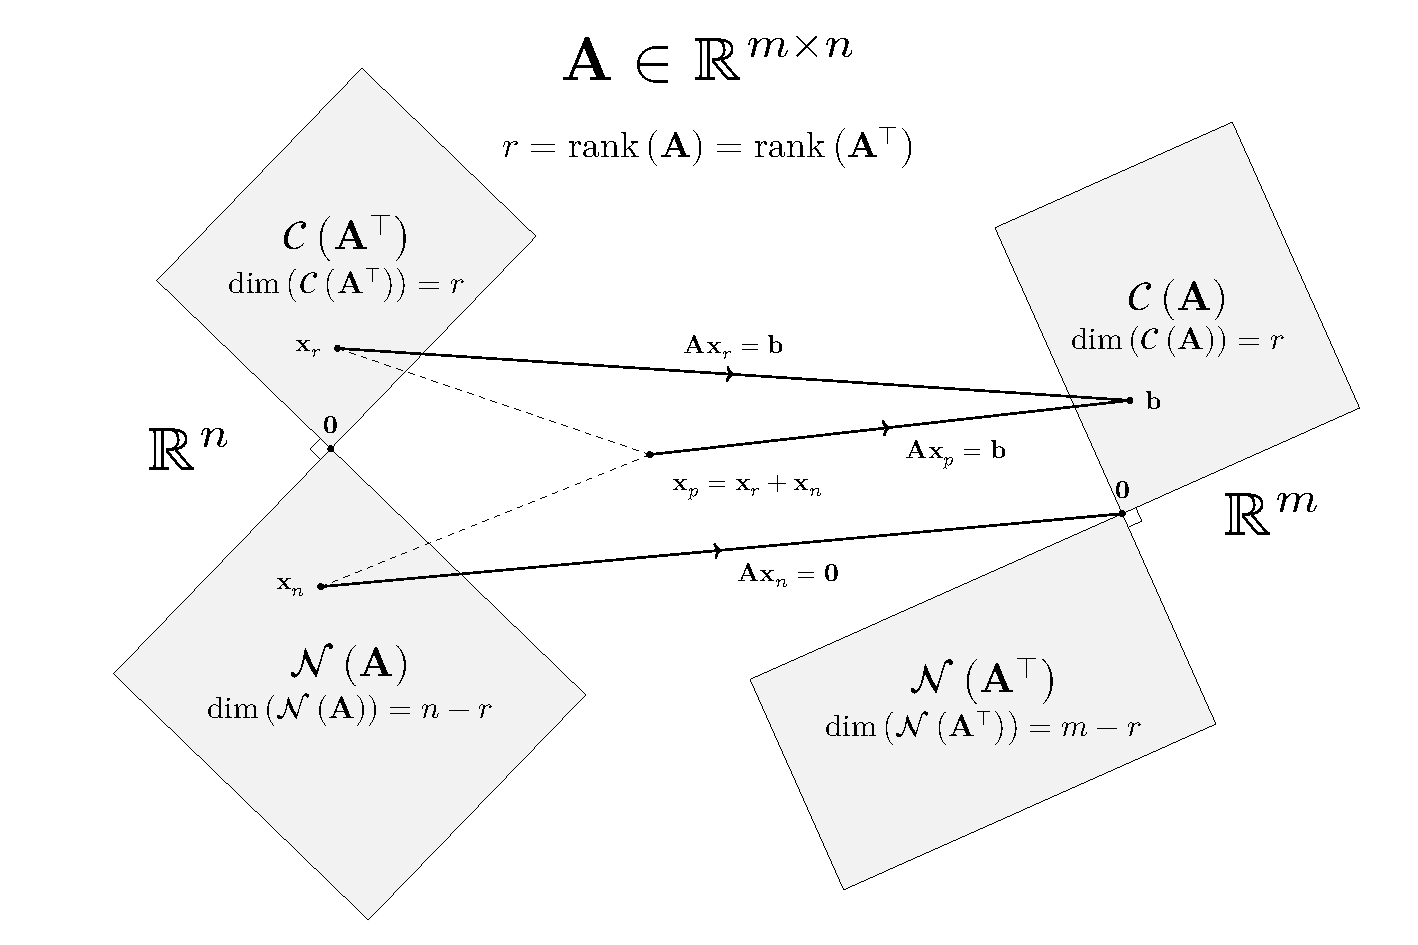
\includegraphics[height = 8cm, keepaspectratio = true]{figures/fundamental_subspaces.pdf}
    \caption{The four fundamental subspaces.} % \label{}
\end{figure}
\subsubsection{Dimensions of Subspaces}
For any matrix \(\symbf{A} \in \R^{m \times n}\):
\begin{definition}[Rank]
    The dimension of the row space is called the \textbf{rank} of a matrix.
    \begin{equation*}
        \vrank{\left( \symbf{A} \right)} = \dim{\left( \rowspace{A} \right)} = r.
    \end{equation*}
    To determine the rank, we can count the number of basic variables in \(\symbf{R}\).
    Note that the rank of \(\symbf{A}\) is equal to the rank of \(\symbf{A}^\top\), so that
    \begin{equation*}
        \vrank{\left( \symbf{A}^\top \right)} = \dim{\left( \columnspace{A} \right)} = r.
    \end{equation*}
\end{definition}
\begin{definition}[Nullity]
    The dimension of the null space is called the \textbf{nullity} of a matrix.
    \begin{equation*}
        \nullity{\left( \symbf{A} \right)} = \dim{\left( \nullspace{A} \right)}.
    \end{equation*}
\end{definition}
\begin{definition}[Left nullity]
    The dimension of the left null space is called the \textbf{left nullity} of the matrix.
    \begin{equation*}
        \nullity{\left( \symbf{A}^\top \right)} = \dim{\left( \leftnullspace{A} \right)}.
    \end{equation*}
\end{definition}
\begin{theorem}[Rank-nullity theorem]
    The dimension of the domain of \(\symbf{A}\), \(\R^n\), is given by
    the sum of the dimensions of the row space and null space of \(\symbf{A}\).
    \begin{align*}
        \dim{\left( \rowspace{A} \right)} + \dim{\left( \nullspace{A} \right)} & = \dim{\left( \R^n \right)} \\
        \vrank{\left( \symbf{A} \right)} + \nullity{\left( \symbf{A} \right)}  & = n                         \\
        r + \nullity{\left( \symbf{A} \right)}                                 & = n.
    \end{align*}
    Therefore,
    \begin{equation*}
        \nullity{\left( \symbf{A} \right)} = n - r.
    \end{equation*}
\end{theorem}
\begin{corollary}[Rank-nullity theorem for the transpose]
    The dimension of the codomain of \(\symbf{A}\), \(\R^m\), is given by
    the sum of the dimensions of the column space and left-null space of \(\symbf{A}\).
    \begin{align*}
        \dim{\left( \columnspace{A} \right)} + \dim{\left( \leftnullspace{A} \right)}   & = \dim{\left( \R^m \right)} \\
        \vrank{\left( \symbf{A}^\top \right)} + \nullity{\left( \symbf{A}^\top \right)} & = m                         \\
        r + \nullity{\left( \symbf{A}^\top \right)}                                     & = m.
    \end{align*}
    Therefore,
    \begin{equation*}
        \nullity{\left( \symbf{A}^\top \right)} = m - r.
    \end{equation*}
\end{corollary}
\begin{theorem}[Orthogonality of subspaces]
    The row space and null space are orthogonal complements in \(\R^n\).
    \begin{equation*}
        \rowspace{A}^\perp = \nullspace{A}
    \end{equation*}
    Similarly, the column space and left-null space are orthogonal complements in \(\R^m\).
    \begin{equation*}
        \columnspace{A}^\perp = \leftnullspace{A}
    \end{equation*}
\end{theorem}
\subsection{Consistency of a Linear System}
Given a matrix \(\symbf{A} \in \R^{m \times n}\) with any vector
\(\symbf{b} \in \R^m\), the linear system \(\symbf{A}\symbf{x} =
\symbf{b}\), can be described as:
\begin{enumerate}
    \item Consistent with a unique solution:
          \begin{equation*}
              \vrank{\left( \symbf{A} \right)} =
              \vrank{\left(
                  \begin{bmatrix}[c|c]
                      \symbf{A} & \symbf{b}
                  \end{bmatrix}
                  \right)} = n
          \end{equation*}
    \item Consistent with infinitely many solutions:
          \begin{equation*}
              \vrank{\left( \symbf{A} \right)} =
              \vrank{\left(
                  \begin{bmatrix}[c|c]
                      \symbf{A} & \symbf{b}
                  \end{bmatrix}
                  \right)} < n
          \end{equation*}
    \item Inconsistent with no solutions:
          \begin{equation*}
              \vrank{\left( \symbf{A} \right)} \neq
              \vrank{\left(
                  \begin{bmatrix}[c|c]
                      \symbf{A} & \symbf{b}
                  \end{bmatrix}
                  \right)}
          \end{equation*}
\end{enumerate}
Note that if \(\symbf{b} \in \columnspace{{A}}\), this system must be
consistent.
\subsection{General Solution to a Linear System}
When \(\symbf{b} \in \columnspace{A}\), the general solution to a
system can be expressed as
\begin{equation*}
    \symbf{x}_g = \symbf{x}_p + \symbf{x}_{ng}
\end{equation*}
where \(\symbf{x}_p \in \R^n\) is a particular solution obtained by
backward substitution, and \(\symbf{x}_{ng} \in \nullspace{A}\) is any
linear combination of the null space basis vectors of
\(\symbf{A}\):
\begin{equation*}
    \symbf{x}_{ng} = \vspan{\left( \leftnullspace{A} \right)}
\end{equation*}
We can do this because:
\begin{align*}
    \symbf{A} \symbf{x}_g & = \symbf{A} \left( \symbf{x}_p + \symbf{x}_{ng} \right)         \\
                          & = \symbf{A} \symbf{x}_p + \symbf{A} \symbf{x}_{ng}              \\
                          & = \symbf{b} + \underbrace{\symbf{A} \symbf{x}_{ng}}_{\symbf{0}} \\
                          & = \symbf{b}
\end{align*}
\subsection{Minimum Norm Solution}
As the particular solution itself is in \(\R^n\), it may also have some
contribution from the null space of \( \symbf{A}\):
\begin{equation*}
    \symbf{x}_p = \symbf{x}_r + \symbf{x}_n, \quad \symbf{x}_r \in \rowspace{A}, \quad \symbf{x}_n \in \nullspace{A}.
\end{equation*}
As we have seen, \(\symbf{x}_n\) can be scaled by any constant without
affecting the validity of the solution, potentially increasing the norm
of \(\symbf{x}_p\). To address this, we define the \textit{minimum norm
    solution} as the one that minimises the squared norm of the solution vector:
\begin{equation*}
    \norm{\symbf{x}_p}^2 = \norm{\symbf{x}_r + \symbf{x}_n}^2 = \norm{\symbf{x}_r}^2 + 2 \symbf{x}_r \cdot \symbf{x}_n + \norm{\symbf{x}_n}^2 = \norm{\symbf{x}_r}^2 + \norm{\symbf{x}_n}^2.
\end{equation*}
This minimum can be achieved by setting \(\symbf{x}_n\) to be the
zero vector, restricting the solution to the row space of \(\symbf{A}\),
so that:
\begin{equation*}
    \symbf{x}_p = \symbf{x}_r \in \rowspace{A}.
\end{equation*}
\section{Least Squares}
Consider an inconsistent system \(\symbf{A}\symbf{x} = \symbf{b}\),
where \(\symbf{b} \notin \columnspace{A}\). In this case, we cannot
find a solution \(\symbf{x}\) that satisfies this equation. Instead,
let us consider an approximate solution that minimises the norm of the
residual vector:
\begin{equation*}
    \norm{\symbf{b} - \symbf{A}\symbf{x}}.
\end{equation*}
This can be expressed as the following optimisation problem:
\begin{equation*}
    \symbf{x} = \argmin_{\symbf{x}^\ast \in \R^n} \norm{\symbf{b} - \symbf{A}\symbf{x}^\ast}
\end{equation*}
which is known as the \textbf{Least Squares} problem.
\begin{theorem}[Minimum norm solution]
    The solution to the least squares problem is obtained when
    \(\symbf{b} - \symbf{A}\symbf{x}\) is orthogonal to the column space of \(\symbf{A}\).
\end{theorem}
\begin{proof}
    Consider the projection of \(\symbf{b}\) onto the column space of
    \(\symbf{A}\):
    \begin{equation*}
        \symbf{b}_P = \proj_{\columnspace{A}} \left( \symbf{b} \right).
    \end{equation*}
    By definition, the residual vector \(\symbf{b} - \symbf{b}_P\)
    is orthogonal to the column space of \(\symbf{A}\). Let
    \(\symbf{w} \neq \symbf{b}_P\) be another vector which also lies in
    the column space of \(\symbf{A}\). Let us compare the difference of
    this vector with the projection vector:
    \begin{equation*}
        \symbf{b} - \symbf{w} = \left( \symbf{b} - \symbf{b}_P \right) + \left( \symbf{b}_P - \symbf{w} \right)
    \end{equation*}
    Taking the squared norm of both sides, noting that
    \(\symbf{b} - \symbf{b}_P\) is orthogonal to \(\symbf{b}_P - \symbf{w}\):
    \begin{align*}
        \norm{\symbf{b} - \symbf{w}}^2 & = \norm{\symbf{b} - \symbf{b}_P}^2 + 2 \left( \symbf{b} - \symbf{b}_P \right) \cdot \left( \symbf{b}_P - \symbf{w} \right) + \norm{\symbf{b}_P - \symbf{w}}^2 \\
                                       & = \norm{\symbf{b} - \symbf{b}_P}^2 + \norm{\symbf{b}_P - \symbf{w}}^2.
    \end{align*}
    Now, as \(\symbf{w}\) was chosen to be different from
    \(\symbf{b}_P\), \(\norm{\symbf{b}_P - \symbf{w}}^2 > 0\). This
    implies,
    \begin{align*}
        \norm{\symbf{b} - \symbf{w}}^2 & > \norm{\symbf{b} - \symbf{b}_P}^2 \\
        \norm{\symbf{b} - \symbf{w}} & > \norm{\symbf{b} - \symbf{b}_P}.
    \end{align*}
    Therefore, if we choose \(\symbf{x}\) to satisfy
    \(\symbf{A} \symbf{x} = \symbf{b}_P\), the residual vector
    \(\symbf{b} - \symbf{A}\symbf{x}\) will be orthogonal to the column
    space of \(\symbf{A}\), and \(\symbf{x}\) will be the minimum norm
    solution to the least squares problem.
\end{proof}
\subsection{Normal Equations}
Given that \(\symbf{b} - \symbf{A}\symbf{x}\) is orthogonal to
\(\columnspace{A}\), it must lie in the left-null space of
\(\symbf{A}\). By orthogonality, we form the following relationship
\begin{equation*}
    \symbf{A}^\top \left( \symbf{b} - \symbf{A}\symbf{x} \right) = \symbfup{0}
\end{equation*}
which is equivalent to solving
\begin{equation*}
    \symbf{A}^\top \symbf{A}\symbf{x} = \symbf{A}^\top \symbf{b}.
\end{equation*}
This linear system is known as the \textbf{Normal Equations} and is
always consistent. It can be thought of as a generalisation of
\(\symbf{A}\symbf{x} = \symbf{b}\) which is not always consistent. Note
that if \(\symbf{b} \in \columnspace{A}\), then the normal equations
produce the same solution as the original system.
\subsection{Orthogonal Projection}
By rearranging the normal equations, we can directly compute the
solution vector:
\begin{equation*}
    \symbf{x} = \left( \symbf{A}^\top \symbf{A} \right)^{-1} \symbf{A}^\top \symbf{b}.
\end{equation*}
The projection of \(\symbf{b}\) onto \(\columnspace{A}\) is therefore
\begin{align*}
    \symbf{b}_P & = \proj_{\columnspace{A}} \left( \symbf{b} \right)                                \\
                & = \symbf{A} \symbf{x}                                                             \\
                & = \symbf{A} \left( \symbf{A}^\top \symbf{A} \right)^{-1} \symbf{A}^\top \symbf{b}
\end{align*}
We can define the matrix
\begin{equation*}
    \symbf{P} = \symbf{A} \left( \symbf{A}^\top \symbf{A} \right)^{-1} \symbf{A}^\top
\end{equation*}
as the orthogonal projector onto the column space of \(\symbf{A}\), so that it operates on \(\symbf{b}\):
\begin{equation*}
    \symbf{P} \symbf{b} = \proj_{\columnspace{A}} \left( \symbf{b} \right)
\end{equation*}
\begin{definition}[Idempotent]
    A matrix \(\symbf{P}\) is idempotent if it satisfies
    \begin{equation*}
        \symbf{P}^2 = \symbf{P}
    \end{equation*}
\end{definition}
Given that \(\symbf{P}\symbf{b}\) produces the projection vector \(\symbf{b}_P\),
taking the orthogonal projection of \(\symbf{b}_P\) again results in the
same projection vector \(\symbf{b}_P\):
\begin{align*}
    \symbf{P} \symbf{b}_P        & = \symbf{b}_P         \\
    \symbf{P}\symbf{P} \symbf{b} & = \symbf{P} \symbf{b} \\
    \symbf{P}^2 \symbf{b}        & = \symbf{P} \symbf{b}.
\end{align*}
\begin{theorem}
    Orthogonal projectors are idempotent matrices.
\end{theorem}
\begin{proof}
    If we express the orthogonal projector in its full form, we can verify the result from above:
    \begin{align*}
        \symbf{P}^2 & = \symbf{P} \symbf{P}                                                                                                                                           \\
                    & = \symbf{A} \left( \symbf{A}^\top \symbf{A} \right)^{-1} \symbf{A}^\top \symbf{A} \left( \symbf{A}^\top \symbf{A} \right)^{-1} \symbf{A}^\top                   \\
                    & = \symbf{A} \cancel{\left( \symbf{A}^\top \symbf{A} \right)^{-1}} \cancel{\symbf{A}^\top \symbf{A}} \left( \symbf{A}^\top \symbf{A} \right)^{-1} \symbf{A}^\top \\
                    & = \symbf{A} \left( \symbf{A}^\top \symbf{A} \right)^{-1} \symbf{A}^\top                                                                                         \\
                    & = \symbf{P}.
    \end{align*}
\end{proof}
\subsection{Dependent Columns}
If \(\symbf{A}\) has dependent columns, then we will obtain an infinite
family of Least Squares solutions. However, there will only be one
projection vector \(\symbf{b}_P\).
This arises from \(\nullspace{A} = \mathcal{N}\left(\symbf{A}^\top
\symbf{A}\right)\), so that the solution to the Normal Equations yields
\begin{equation*}
    \symbf{x} = \symbf{x}_p + \symbf{x}_{ng}
\end{equation*}
where \(\symbf{x}_p\) is the particular Least Squares solution, and \(\symbf{x}_{ng}\) represents
any linear combination of null space vectors.
\subsection{Orthogonal Projector onto the Column Space}
To obtain a unique solution to the Normal Equations, we can form the
matrix \(\symbf{W}\) such that it has full column rank, and it spans the
column space of \(\symbf{A}\). Then the orthogonal projector is given
by
\begin{equation*}
    \symbf{P} = \symbf{W} \left( \symbf{W}^\top \symbf{W} \right)^{-1} \symbf{W}^\top
\end{equation*}
\subsection{Orthogonal Projectors onto other Spaces}
Given the orthogonal projector \(\symbf{P} = \proj_V\) onto a subspace
\(V\), the orthogonal projector \(\symbf{Q} = \proj_{V^\perp}\) onto
\(V^\perp\) is given by
\begin{equation*}
    \symbf{Q} = \symbf{I} - \symbf{P}
\end{equation*}
This is because the vector \(\symbf{b}\) can be represented as the
sum of the projections onto \(V\) and \(V^\perp\)
\begin{equation*}
    \symbf{b} = \symbf{P}\symbf{b} + \symbf{Q}\symbf{b}.
\end{equation*}
The dot product of these two vectors is therefore also zero, given that
both projections lie in orthogonal subspaces.
\begin{equation*}
    \left( \symbf{P}\symbf{b} \right)^\top \symbf{Q}\symbf{b} = \symbf{0}
\end{equation*}
or
\begin{equation*}
    \symbf{P} \symbf{Q} = \symbf{0}
\end{equation*}
where \(\symbf{0}\) is the zero matrix.
\section{Orthogonal Matrices}
\subsection{Standard Basis Vectors}
The standard basis vectors are constructed by placing a \(1\) in the
\(n\)th row of the \(n\)th basis vector in \(\R^n\).
\begin{equation*}
    \symbf{e}_1 =
    \begin{bmatrix}
        1      \\
        0      \\
        \vdots \\
        0
    \end{bmatrix}
    ,\: \dots,\: \symbf{e}_n =
    \begin{bmatrix}
        0      \\
        0      \\
        \vdots \\
        1
    \end{bmatrix}
\end{equation*}
\subsection{Standard Basis}
In \(\R^n\), the standard basis \(S\) consists of the vectors
\begin{equation*}
    S = \left\{ \symbf{e}_1,\: \dots,\: \symbf{e}_n \right\}
\end{equation*}
where the coefficients of a column vector implicitly represent the coefficients
of the linear \linebreak combination of basis vectors in \(S\).
For example, the vector \(\symbf{b}\) in the standard basis
\begin{equation*}
    \symbf{b} = b_1 \symbf{e}_1 + \cdots + b_n \symbf{e}_n
\end{equation*}
can be explicitly represented as a column vector
\begin{equation*}
    \left( \symbf{b} \right)_S =
    \begin{bmatrix}
        b_1    \\
        \vdots \\
        b_n
    \end{bmatrix}
\end{equation*}
where \(b_1,\: \dots,\: b_n\) are the entries of \(\left( \symbf{b} \right)_S\) with respect to the standard basis \(S\).
\subsection{Change of Basis}
To represent the vector \(\symbf{b}\) in terms of another basis \(W\),
where
\begin{equation*}
    W = \left\{ \symbf{w}_1,\: \dots,\: \symbf{w}_n \right\}
\end{equation*}
we must determine the components of each basis vector in \(W\) that
contributes to \(\symbf{b}\). This is represented by the system:
\begin{align*}
    \symbf{b} & = c_1 \symbf{w}_1 + \cdots + c_n \symbf{w}_n \\
    \symbf{b} & =
    \begin{bmatrix}
        \vertbar    &        & \vertbar    \\
        \symbf{w}_1 & \cdots & \symbf{w}_n \\
        \vertbar    &        & \vertbar
    \end{bmatrix}
    \begin{bmatrix}
        c_1    \\
        \vdots \\
        c_n
    \end{bmatrix}
    \\
    \symbf{b} & = \symbf{W} \symbf{c}
\end{align*}
The component vector \(\symbf{c}\) is precisely the representation of \(\symbf{b}\)
with respect to the basis \(W\), so that
\begin{equation*}
    \left( \symbf{b} \right)_W = \symbf{c}.
\end{equation*}
\subsection{Orthonormal Basis}
If we consider a basis \(Q\), such that every basis vector is
normalised and orthogonal to every other basis vector, then \(Q\) is an
orthonormal basis.
\begin{definition}[Kronecker delta]
    We can summarise such a basis using the Kronecker delta \(\delta_{ij}\),
    which is defined
    \begin{equation*}
        \delta_{ij} =
        \begin{cases}
            1, & i = j   \\
            0, & i \ne j
        \end{cases}
    \end{equation*}
    so that in an orthonormal basis \(Q\) with basis vectors
    \(\left\{ \symbf{q}_1,\: \dots,\: \symbf{q}_n \right\}\)
    \begin{equation*}
        \symbf{q}_i^\top \symbf{q}_j = \delta_{ij}
    \end{equation*}
\end{definition}
By using an orthonormal basis, we can determine the coefficients of \(\left( \symbf{b} \right)_Q\) without
the need to solve a linear system. For example, the \(i\)th coefficient can be determined as
follows
\begin{align*}
    \symbf{b}                  & = c_1 \symbf{q}_1 + \cdots + c_n \symbf{q}_n                                                                                                                         \\
    \symbf{q}_i^\top \symbf{b} & = \symbf{q}_i^\top \left( c_1 \symbf{q}_1 + \cdots + c_i \symbf{q}_i + \cdots + c_n \symbf{q}_n \right)                                                              \\
    \symbf{q}_i^\top \symbf{b} & = c_1 \cancelto{0}{\symbf{q}_i^\top \symbf{q}_1} + \cdots + c_i \cancelto{1}{\symbf{q}_i^\top \symbf{q}_i} + \cdots + c_n \cancelto{0}{\symbf{q}_i^\top \symbf{q}_n} \\
    \symbf{q}_i^\top \symbf{b} & = c_i                                                                                                                                                                \\
    \symbf{Q}^\top \symbf{b}   & = \symbf{c}
\end{align*}
Therefore
\begin{align*}
    \left( \symbf{b} \right)_Q & = \symbf{Q}^\top \symbf{b}
\end{align*}
\subsection{Orthogonal Matrices}
To confirm that \(Q = \left\{ \symbf{q}_1,\: \dots,\: \symbf{q}_n
\right\}\) is an orthonormal basis, we need to confirm that
\(\symbf{q}_i^\top \symbf{q}_j = \delta_{ij}\) holds for all basis
vectors \(\symbf{q}_i\). To do so, we can construct the matrix product
\(\symbf{Q}^\top \symbf{Q}\), so that
\begin{align*}
    \symbf{Q}^\top \symbf{Q} & =
    \begin{bmatrix}
        \horzbar & \symbf{q}_1 & \horzbar \\
                 & \vdots                 \\
        \horzbar & \symbf{q}_n & \horzbar
    \end{bmatrix}
    \begin{bmatrix}
        \vertbar    &        & \vertbar    \\
        \symbf{q}_1 & \cdots & \symbf{q}_n \\
        \vertbar    &        & \vertbar
    \end{bmatrix}
    \\
                             & =
    \begin{bmatrix}
        \symbf{q}_1^\top \symbf{q}_1 & \cdots & \symbf{q}_1^\top\symbf{q}_n  \\
        \vdots                       & \ddots & \vdots                       \\
        \symbf{q}_n^\top \symbf{q}_1 & \cdots & \symbf{q}_n^\top \symbf{q}_n
    \end{bmatrix}
    \\
                             & =
    \begin{bmatrix}
        1      & 0      & \cdots & 0      \\
        0      & 1      & \ddots & \vdots \\
        \vdots & \ddots & \ddots & 0      \\
        0      & \cdots & 0      & 1
    \end{bmatrix}
    \\
                             & = \symbf{I}.
\end{align*}
\begin{definition}[Orthogonal Matrices]
    A square matrix \(\symbf{Q}\) is \textit{orthogonal} if it satisfies
    \begin{equation*}
        \symbf{Q}^\top = \symbf{Q}^{-1}
    \end{equation*}
    so that
    \begin{equation*}
        \symbf{Q}^\top \symbf{Q} = \symbf{Q}\symbf{Q}^\top = \symbf{I}.
    \end{equation*}
\end{definition}
\subsection{Projection onto a Vector}
Consider a subspace which consists of one vector \(\symbf{a}\), the
projection of \(\symbf{b}\) onto \(\symbf{a}\) is given by
\begin{align*}
    \proj_{\symbf{a}} \left( \symbf{b} \right) = \symbf{b}_P & = \symbf{a} \left( \symbf{a}^\top \symbf{a} \right)^{-1} \symbf{a}^\top \symbf{b} \\
                                                             & = \frac{\symbf{a}}{\norm{\symbf{a}}^2} \symbf{a} \cdot \symbf{b}
\end{align*}
If we instead project \(\symbf{b}\) onto a unit vector \(\symbf{q}\), then this simplifies to
\begin{equation*}
    \proj_{\symbf{q}} \left( \symbf{b} \right) = \symbf{q} \left( \symbf{q} \cdot \symbf{b} \right)
\end{equation*}
\subsection{Gram-Schmidt Process}
To convert an arbitrary basis \(W\)\footnote{Here we use \(W\) to
denote the set of vectors that span \(\columnspace{A}\).} to an
orthonormal basis \(Q\), we must develop a process that is
generalisable to any basis.
We construct \(Q\) as follows
\begin{align*}
    \symbf{v}_1 & = \symbf{w}_1                                                                                                   & \symbf{q}_1 & = \frac{\symbf{v}_1}{\norm{\symbf{v}_1}}  \\
    \symbf{v}_2 & = \symbf{w}_2 - \proj_{\symbf{q}_1} \left( \symbf{w}_2 \right)                                                  & \symbf{q}_2 & = \frac{\symbf{v}_2}{\norm{\symbf{v}_2}}  \\
    \symbf{v}_3 & = \symbf{w}_3 - \proj_{\symbf{q}_1} \left( \symbf{w}_3 \right) - \proj_{\symbf{q}_2} \left( \symbf{w}_3 \right) & \symbf{q}_3 & = \frac{\symbf{v}_3}{\norm{\symbf{v}_3}}  \\
                & \vdotswithin{=}                                                                                                 &             & \vdotswithin{=}                           \\
    \symbf{v}_i & = \symbf{w}_i - \sum_{j = 1}^{i - 1} \proj_{\symbf{q}_j} \left( \symbf{w}_i \right)                             & \symbf{q}_i & = \frac{\symbf{v}_i}{\norm{\symbf{v}_i}}.
\end{align*}
Using the projection definition for orthogonal vectors, we can simplify this to
\begin{align*}
    \symbf{v}_1 & = \symbf{w}_1                                                                                                                       & \symbf{q}_1 & = \frac{\symbf{v}_1}{\norm{\symbf{v}_1}}  \\
    \symbf{v}_2 & = \symbf{w}_2 - \symbf{q}_1 \left( \symbf{q}_1 \cdot \symbf{w}_2 \right)                                                            & \symbf{q}_2 & = \frac{\symbf{v}_2}{\norm{\symbf{v}_2}}  \\
    \symbf{v}_3 & = \symbf{w}_3 - \symbf{q}_1 \left( \symbf{q}_1 \cdot \symbf{w}_3 \right) - \symbf{q}_2 \left( \symbf{q}_2 \cdot \symbf{w}_3 \right) & \symbf{q}_3 & = \frac{\symbf{v}_3}{\norm{\symbf{v}_3}}  \\
                & \vdotswithin{=}                                                                                                                     &             & \vdotswithin{=}                           \\
    \symbf{v}_i & = \symbf{w}_i - \sum_{j = 1}^{i - 1} \symbf{q}_j \left( \symbf{q}_j \cdot \symbf{w}_i \right)                                       & \symbf{q}_i & = \frac{\symbf{v}_i}{\norm{\symbf{v}_i}}.
\end{align*}
This produces two sets of mutually orthogonal vectors that span the same space as \(W\). Here \(V = \left\{ \symbf{v}_1,\: \dots,\: \symbf{v}_n \right\}\) is an orthogonal basis,
and \(Q = \left\{ \symbf{q}_1,\: \dots,\: \symbf{q}_n \right\}\) is an orthonormal basis.
\subsection{QR Decomposition}
If we rearrange the steps in the Gram-Schmidt process to solve for
\(\symbf{w}_i\), we get
\begin{align*}
    \symbf{w}_1 & = \symbf{q}_1 \norm{\symbf{v}_1}                                                                                                                       \\
    \symbf{w}_2 & = \symbf{q}_2 \norm{\symbf{v}_2} + \symbf{q}_1 \left( \symbf{q}_1 \cdot \symbf{w}_2 \right)                                                            \\
    \symbf{w}_3 & = \symbf{q}_3 \norm{\symbf{v}_3} + \symbf{q}_1 \left( \symbf{q}_1 \cdot \symbf{w}_3 \right) + \symbf{q}_2 \left( \symbf{q}_2 \cdot \symbf{w}_3 \right) \\
                &                                                                                                                                                        \\
    \symbf{w}_i & = \symbf{q}_i \norm{\symbf{v}_i} + \sum_{j = 1}^{i - 1} \symbf{q}_j \left( \symbf{q}_j \cdot \symbf{w}_i \right)
\end{align*}
Due to the properties of \(\symbf{q}_i\), we can also express \(\symbf{w}_i\) as
\begin{equation*}
    \symbf{w}_i = \sum_{j = 1}^{i} \symbf{q}_j \left( \symbf{q}_j \cdot \symbf{w}_i \right).
\end{equation*}
And in vector form:
\begin{align*}
    \begin{bmatrix}
        \symbf{w}_1 & \symbf{w}_2 & \cdots & \symbf{w}_n
    \end{bmatrix}
              & =
    \begin{bmatrix}
        \symbf{q}_1 & \symbf{q}_2 & \cdots & \symbf{q}_n
    \end{bmatrix}
    \begin{bmatrix}
        \norm{\symbf{v}_1} & \symbf{q}_1 \cdot \symbf{w}_2 & \cdots & \symbf{q}_1 \cdot \symbf{w}_n       \\[0.2cm]
        0                  & \norm{\symbf{v}_2}            & \ddots & \vdots                              \\[0.2cm]
        \vdots             & \ddots                        & \ddots & \symbf{q}_{n - 1} \cdot \symbf{w}_n \\[0.2cm]
        0                  & \cdots                        & 0      & \norm{\symbf{v}_n}
    \end{bmatrix}
    \\
    \symbf{W} & = \symbf{Q} \symbf{R}
\end{align*}
\subsection{Least Squares using QR Decomposition}
Consider \(\symbf{u} \notin \columnspace{A}\), by using the QR
decomposition of \(\symbf{A}\), we have
\begin{align*}
    \symbf{A} \symbf{c}                          & = \symbf{u}                 \\
    \left( \symbf{Q} \symbf{R} \right) \symbf{c} & = \symbf{u}                 \\
    \symbf{Q}^\top \symbf{Q} \symbf{R} \symbf{c} & = \symbf{Q}^\top \symbf{u}  \\
    \symbf{R} \symbf{c}                          & = \symbf{Q}^\top \symbf{u}.
\end{align*}
Alternatively, consider the Normal Equations,
\begin{align*}
    \symbf{A}^\top \symbf{A} \symbf{c}                                                   & = \symbf{A}^\top \symbf{u}                                                   \\
    \left( \symbf{Q} \symbf{R} \right)^\top \left( \symbf{Q} \symbf{R} \right) \symbf{c} & = \left( \symbf{Q} \symbf{R} \right)^\top \symbf{u}                          \\
    \symbf{R}^\top \symbf{Q}^\top \symbf{Q} \symbf{R} \symbf{c}                          & = \symbf{R}^\top \symbf{Q}^\top \symbf{u}                                    \\
    \symbf{R}^\top \symbf{R} \symbf{c}                                                   & = \symbf{R}^\top \symbf{Q}^\top \symbf{u}                                    \\
    \left( \symbf{R}^\top \right)^{-1} \symbf{R}^\top \symbf{R} \symbf{c}                & = \left( \symbf{R}^\top \right)^{-1} \symbf{R}^\top \symbf{Q}^\top \symbf{u} \\
    \symbf{R} \symbf{c}                                                                  & = \symbf{Q}^\top \symbf{u}
\end{align*}
Therefore by using the QR decomposition of \(\symbf{A}\) we can find the Least Squares solution \(\symbf{c}^\ast\), using backward-substitution.
\section{Eigenvalues and Eigenvectors}
\subsection{Linear Operators}
Consider the linear transformation \(T\) that maps any vector
\(\symbf{v}\in V\) to \(V\). \(T\) is referred to as a linear operator
from \(V\) to \(V\):
\begin{equation*}
    T:V \to V.
\end{equation*}
\subsection{The Eigenvalue Problem}
Given the linear transformation
\begin{equation*}
    \symbf{v} \mapsto \symbf{A} \symbf{v}
\end{equation*}
for \(\symbf{A}\in\R^{n \times n}\), let \(\symbf{v}\) be an eigenvector of \(\symbf{A}\)
and \(\lambda\) its associated eigenvalue so that the following relationship is
satisfied,
\begin{equation*}
    \symbf{A}\symbf{v} = \lambda \symbf{v}.
\end{equation*}
These eigenvalue and eigenvector pairs form eigenpairs of \(\symbf{A}\).
\subsection{Calculating Eigenvalues}
By rearranging the eigenvalue problem we have,
\begin{align*}
    \symbf{A}\symbf{v}                                    & = \lambda \symbf{v}           \\
    \symbf{A}\symbf{v}                                    & = \lambda \symbf{I} \symbf{v} \\
    \lambda \symbf{I} \symbf{v} - \symbf{A}\symbf{v}      & = \symbf{0}                   \\
    \left( \lambda \symbf{I} - \symbf{A} \right)\symbf{v} & = \symbf{0}.
\end{align*}
For this homogeneous linear system to have non-trivial solutions, the rank of the coefficient matrix \(\lambda \symbf{I} - \symbf{A}\)
must be less than \(n\). This requires the matrix to be singular so that its determinant is equal to \(0\):
\begin{equation*}
    \det{\left( \lambda \symbf{I} - \symbf{A} \right)} = 0.
\end{equation*}
\begin{definition}[Characteristic polynomial]
    Let \(P\left( \lambda \right)\) denote the resulting polynomial of degree \(n\):
    \begin{equation*}
        P\left( \lambda \right) = \det{\left( \lambda \symbf{I} - \symbf{A} \right)}.
    \end{equation*}
\end{definition}
We use \(\lambda \symbf{I} - \symbf{A}\) rather than \(\symbf{A} - \lambda \symbf{I}\) to ensure that the polynomial is monic,
i.e.\ the leading coefficient is equal to \(1\).
\subsection{Calculating Eigenvectors}
To calculate the eigenvector \(\symbf{v}_i\) associated with the
eigenvalue \(\lambda_i\), we must find the null space of \(\lambda_i
\symbf{I} - \symbf{A}\). As this yields a basis for the null space, any
scalar multiple of an eigenvalue also satisfies the eigenvalue problem.
\begin{definition}[Eigenspace]
    The null space of \(\lambda_i \symbf{I} - \symbf{A}\) is called the eigenspace associated with \(\lambda_i\).
\end{definition}
\subsection{Eigen Decomposition}
The equations formed by all eigenpairs of the matrix \(\symbf{A}\) can
be expressed as
\begin{equation*}
    \symbf{A} \symbf{V} = \symbf{V} \symbf{D}
\end{equation*}
which gives us the eigendecomposition or diagonalisation of \(\symbf{A}\),
\begin{equation*}
    \symbf{A} = \symbf{V} \symbf{D} \symbf{V}^{-1}.
\end{equation*}
Here \(\symbf{V}\) is a matrix comprised of the eigenvectors \(\symbf{v}_i\) as its columns, and \(\symbf{D}\) is a
diagonal matrix of the eigenvalues \(\lambda_i\). Mathematically,
\begin{align*}
    \symbf{V} & =
    \begin{bmatrix}
        \symbf{v}_1 & \cdots & \symbf{v}_n
    \end{bmatrix}
              & \symbf{D} & = \diag{\left( \lambda_1,\: \dots,\: \lambda_n \right)}
\end{align*}
\begin{definition}[Algebraic multiplicity]
    The algebraic multiplicity \(\mu_{\symbf{A}}\left( \lambda_i \right)\)
    of an eigenvalue \(\lambda_i\) is
    the multiplicity of \(\lambda_i\) in the characteristic polynomial
    (i.e.,\ how many times it is repeated).
    For \(d \leq n\) distinct eigenvalues,
    \begin{equation*}
        P\left( \lambda \right) = 0 = \left( \lambda - \lambda_1 \right)^{\mu_{\symbf{A}}\left( \lambda_1 \right)} \left( \lambda - \lambda_2 \right)^{\mu_{\symbf{A}}\left( \lambda_2 \right)} \cdots \left( \lambda - \lambda_d \right)^{\mu_{\symbf{A}}\left( \lambda_d \right)}.
    \end{equation*}
    This requires
    \begin{gather*}
        1 \leq \mu_{\symbf{A}}\left( \lambda_i \right) \leq n         \\
        \mu_{\symbf{A}} = \sum_{i = 1}^d \mu_{\symbf{A}} \left( \lambda_i \right) = n
    \end{gather*}
\end{definition}
\begin{definition}[Geometric multiplicity]
    The dimension of the eigenspace associated with \(\lambda_i\) is referred to as the
    geometric multiplicity of \(\lambda_i\), denoted \(\gamma_{\symbf{A}}\left( \lambda_i \right)\).
    As the eigenspace is by definition the null space of \(\lambda_i
    \symbf{I} - \symbf{A}\),
    \begin{equation*}
        \gamma_{\symbf{A}} \left( \lambda_i \right) = \nullity{\left( \lambda_i \symbf{I} - \symbf{A} \right)}.
    \end{equation*}
    Given \(d \leq n\) distinct eigenvalues,
    \begin{gather*}
        1 \leq \gamma_{\symbf{A}}\left( \lambda_i \right) \leq \mu_{\symbf{A}}\left( \lambda_i \right) \leq n \\
        \gamma_{\symbf{A}} = \sum_{i = 1}^d \gamma_{\symbf{A}} \left( \lambda_i \right)
    \end{gather*}
    so that
    \begin{equation*}
        d \leq \gamma_{\symbf{A}} \leq n.
    \end{equation*}
\end{definition}
\begin{theorem}[Eigenvectors of distinct eigenvalues]
    Eigenvectors corresponding to distinct eigenvalues are linearly dependent.
\end{theorem}
\begin{definition}[Defective matrix]
    A defective matrix is a matrix that does not have a complete basis of eigenvectors and is therefore not diagonalisable.
    In particular, there exists at least one eigenvalue \(\lambda_k\),
    where \(\gamma_{\symbf{A}}\left( \lambda_k \right) < \mu_{\symbf{A}}\left( \lambda_k \right)\)
\end{definition}
\subsection{Matrix Similarity}
\begin{definition}[Similar matrices]
    Two \(n \times n\) matrices \(\symbf{A}\) and \(\symbf{B}\) are similar,
    if there exists an invertible \(n \times n\) matrix \(\symbf{P}\) such that
    \begin{equation*}
        \symbf{B} = \symbf{P}^{-1} \symbf{A} \symbf{P}.
    \end{equation*}
\end{definition}
\begin{theorem}[Characteristic polynomial of similar matrices]
    Two similar matrices \(\symbf{A}\) and \(\symbf{B}\) have the
    same characteristic polynomial \(P\left( \lambda \right)\) so that they share their ranks,
    determinants, trace, and eigenvalues (including their algebraic and geometric multiplicities).
\end{theorem}
\begin{proof}
    The eigenvalues of \(\symbf{B}\) can be determined using the characteristic polynomial:
    \begin{align*}
        P_{\symbf{B}}\left( \lambda \right) & = \det{\left( \lambda \symbf{I} - \symbf{B} \right)}                                                                    \\
                                            & = \det{\left( \lambda \symbf{I} - \symbf{P}^{-1} \symbf{A} \symbf{P} \right)}                                           \\
                                            & = \det{\left( \lambda \symbf{P}^{-1} \symbf{I} \symbf{P} - \symbf{P}^{-1} \symbf{A} \symbf{P} \right)}                  \\
                                            & = \det{\left( \symbf{P}^{-1} \left( \lambda \symbf{I} - \symbf{A} \right) \symbf{P} \right)}                            \\
                                            & = \det{\left( \symbf{P}^{-1} \right)} \det{\left( \lambda \symbf{I} - \symbf{A} \right)} \det{\left( \symbf{P} \right)} \\
                                            & = \det{\left( \symbf{P}^{-1} \symbf{P} \right)} \det{\left( \lambda \symbf{I} - \symbf{A} \right)}                      \\
                                            & = \det{\left( \symbf{I} \right)} \det{\left( \lambda \symbf{I} - \symbf{A} \right)}                                     \\
                                            & = \det{\left( \lambda \symbf{I} - \symbf{A} \right)}                                                                    \\
                                            & = P_{\symbf{A}}\left( \lambda \right)
    \end{align*}
\end{proof}
\subsection{Constructing a Similar Matrix}
Given a diagonalisable matrix \(\symbf{A} =
\symbf{V}\symbf{D}\symbf{V}^{-1}\), we can construct the matrix
\(\symbf{B}\) with arbitrary eigenvectors \(\symbf{W}\), so that
\begin{align*}
    \symbf{B} = \symbf{W} \symbf{D} \symbf{W}^{-1}.
\end{align*}
Using \(\symbf{D} = \symbf{V}^{-1} \symbf{A} \symbf{V}\),
\begin{align*}
    \symbf{B} & = \symbf{W} \symbf{D} \symbf{W}^{-1}                                               \\
              & = \symbf{W} \left( \symbf{V}^{-1} \symbf{A} \symbf{V} \right) \symbf{W}^{-1}       \\
              & = \left( \symbf{V} \symbf{W}^{-1} \right)^{-1} \symbf{A} \symbf{V} \symbf{W}^{-1}.
\end{align*}
Let \(\symbf{P} = \symbf{V} \symbf{W}^{-1}\), so that
\begin{equation*}
    \symbf{B} = \symbf{P}^{-1} \symbf{A} \symbf{P}.
\end{equation*}
This result shows us that \(\symbf{A}\) and \(\symbf{B}\) are similar matrices.
\subsection{Symmetric Matrices}
Consider the symmetric matrix \(\symbf{A}\in\R^{n \times n}\) where
\(\symbf{A}^\top = \symbf{A}\). Then:
\begin{enumerate}
    \item \(\symbf{A}\) is always diagonalisable.
    \item The eigenvalues and eigenvectors of symmetric matrices are
          always real.
    \item The eigenspaces of a symmetric matrix are orthogonal for
          \(\lambda_i \neq \lambda_j\).
\end{enumerate}
\subsection{Orthogonal Matrices}
By applying the Gram-Schmidt process to the eigenvectors of a symmetric
matrix, we obtain the decomposition
\begin{equation*}
    \symbf{A} = \symbf{Q} \symbf{D} \symbf{Q}^\top
\end{equation*}
where \(\symbf{Q}\) is an orthogonal matrix that satisfies \(\symbf{Q}^{-1} = \symbf{Q}^\top\).
\subsection{Definite Matrices}
Symmetric matrices are also known as definite matrices, and can be
classified into four categories.
\begin{enumerate}
    \item Positive definite matrices: All eigenvalues are positive.
    \item Positive semi-definite matrices: All eigenvalues are
          non-negative.
    \item Negative definite matrices: All eigenvalues are non-positive.
    \item Negative semi-definite matrices: All eigenvalues are negative.
\end{enumerate}
\subsection{Eigenbases}
When \(\symbf{A}\) has \(n\) linearly independent eigenvectors, the
columns of \(\symbf{V}\) represent the eigenbasis of \(\symbf{A}\).
Let the basis \(V\) be the columns of \(\symbf{V}\) so that for the
linear system \(\symbf{A}\symbf{x} = \symbf{b}\), \(\left[ \symbf{x}
\right]_V = \symbf{c}\) and \(\left[ \symbf{b} \right]_V = \symbf{k}\),
then
\begin{align*}
    \symbf{A} \symbf{x}                          & = \symbf{b}                  \\
    \symbf{A} \symbf{V} \symbf{c}                & = \symbf{V} \symbf{k}        \\
    \symbf{V}^{-1} \symbf{A} \symbf{V} \symbf{c} & = \symbf{k}                  \\
    \symbf{D} \symbf{c}                          & = \symbf{k}                  \\
    \symbf{D} \left( \symbf{x} \right)_V         & = \left( \symbf{b} \right)_V
\end{align*}
so that, with respect to the eigenbasis, a linear map from \(\R^n\) to \(\R^n\) is represented by the matrix \(\symbf{D}\).
\subsection{Matrix Functions}
Given a nondefective \(\symbf{A} \in \R^{n \times n}\) with the
eigendecomposition \(\symbf{A} = \symbf{V} \symbf{D} \symbf{V}^{-1}\),
we can form the following equalities.
\subsubsection{Powers}
For \(k \in \N\),
\begin{equation*}
    \symbf{A}^k = \symbf{V} \symbf{D}^k \symbf{V}^{-1} = \symbf{V} \diag{\left( \lambda_1^k,\: \ldots,\: \lambda_n^k \right)} \symbf{V}^{-1}.
\end{equation*}
\begin{proof}
    We can prove the above theorem using a recursive construction of \(\symbf{A}^k\).
    \begin{align*}
        \symbf{A}^2 = \symbf{A} \symbf{A}   & = \symbf{V} \symbf{D} \cancel{\symbf{V}^{-1} \symbf{V}} \symbf{D} \symbf{V}^{-1} = \symbf{V} \symbf{D}^2 \symbf{V}^{-1}   \\
        \symbf{A}^3 = \symbf{A}^2 \symbf{A} & = \symbf{V} \symbf{D}^2 \cancel{\symbf{V}^{-1} \symbf{V}} \symbf{D} \symbf{V}^{-1} = \symbf{V} \symbf{D}^3 \symbf{V}^{-1}
    \end{align*}
    so that for a positive integer \(k \in \N\),
    \begin{equation*}
        \symbf{A}^k = \symbf{A}^{k - 1} \symbf{A} = \symbf{V} \symbf{D}^{k - 1} \cancel{\symbf{V}^{-1} \symbf{V}} \symbf{D} \symbf{V}^{-1} = \symbf{V} \symbf{D}^k \symbf{V}^{-1}.
    \end{equation*}
\end{proof}
\subsubsection{Polynomials}
Let \(p\left( t \right) = c_0 + c_1 t + c_2 t^2 + \cdots + c_k t^k\)
denote a polynomial of degree \(k\), then the matrix polynomial
\(p\left( \symbf{A} \right)\) can be expressed as
\begin{align*}
    p\left( \symbf{A} \right) & = c_0 \symbf{I} + c_1 \symbf{A} + c_2 \symbf{A}^2 + \cdots + c_k \symbf{A}^k                                                                                                     \\
                              & = c_0 \symbf{V} \symbf{I} \symbf{V}^{-1} + c_1 \symbf{V} \symbf{D} \symbf{V}^{-1} + c_2 \symbf{V} \symbf{D}^2 \symbf{V}^{-1} + \cdots + c_k \symbf{V} \symbf{D}^k \symbf{V}^{-1} \\
                              & = \symbf{V} \left( c_0 \symbf{I} + c_1 \symbf{D} + c_2 \symbf{D}^2 + \cdots + c_k \symbf{D}^k \right) \symbf{V}^{-1}                                                             \\
                              & = \symbf{V} p\left( \symbf{D} \right) \symbf{V}^{-1}                                                                                                                             \\
                              & = \symbf{V} \diag{\left( p\left( \lambda_1 \right),\: \ldots,\: p\left( \lambda_n \right) \right)} \symbf{V}^{-1}.
\end{align*}
\subsection{Analytic Functions}
An analytic function can be represented by its Taylor series expansion,
allowing us to operate analytic functions on \(\symbf{A}\).
\begin{align*}
    f\left( \symbf{A} \right) & = \symbf{V} f\left( \symbf{D} \right) \symbf{V}^{-1}                                                               \\
                              & = \symbf{V} \diag{\left( f\left( \lambda_1 \right),\: \ldots,\: f\left( \lambda_n \right) \right)} \symbf{V}^{-1}.
\end{align*}
\begin{theorem}[Cayley-Hamilton theorem]
    The characteristic polynomial of a square matrix \(\symbf{A}\) (that is not necessarily diagonalisable)
    is equal to the zero matrix.
    \begin{equation*}
        P\left( \symbf{A} \right) = \symbfup{0}
    \end{equation*}
\end{theorem}
\section{Singular Value Decomposition}
The singular value decomposition (SVD) of \(\symbf{A} \in \R^{m \times
n}\) is given by
\begin{equation*}
    \symbf{A} = \symbf{U} \symbf{\Sigma} \symbf{V}^\top
\end{equation*}
where \(\symbf{U} \in \R^{m \times m}\) is an orthogonal matrix, \(\symbf{\Sigma} \in \R^{m \times n}\)
is a diagonal matrix, and \(\symbf{V} \in  \R^{n \times n}\) is
an orthogonal matrix.
\(\symbf{U}\) is known as the left-singular matrix and \(\symbf{V}\) is the right-singular matrix,
corresponding to how these matrices are multiplied to \(\symbf{\Sigma}\).
\(\symbf{\Sigma}\) consists of the \textbf{singular values} \(\sigma_i\) of \(\symbf{A}\), which can be determined
using the following process:
\begin{align*}
    \symbf{A}^\top \symbf{A} & = \left( \symbf{U} \symbf{\Sigma} \symbf{V}^\top \right)^\top \left( \symbf{U} \symbf{\Sigma} \symbf{V}^\top \right) \\
                             & = \symbf{V} \symbf{\Sigma}^\top \symbf{U}^\top \symbf{U} \symbf{\Sigma} \symbf{V}^\top                               \\
                             & = \symbf{V} \symbf{\Sigma}^\top \symbf{\Sigma} \symbf{V}^\top
\end{align*}
similarly,
\begin{align*}
    \symbf{A} \symbf{A}^\top & = \left( \symbf{U} \symbf{\Sigma} \symbf{V}^\top \right) \left( \symbf{U} \symbf{\Sigma} \symbf{V}^\top \right)^\top \\
                             & = \symbf{U} \symbf{\Sigma} \symbf{V}^\top \symbf{V} \symbf{\Sigma}^\top \symbf{U}^\top                               \\
                             & = \symbf{U} \symbf{\Sigma} \symbf{\Sigma}^\top \symbf{U}^\top
\end{align*}
In both instances, we form an orthogonal eigendecomposition where
\(\symbf{\Sigma}^\top \symbf{\Sigma}\) and \(\symbf{\Sigma} \symbf{\Sigma}^\top\) are the eigenvalues of
\(\symbf{A}^\top\symbf{A}\) and \(\symbf{A}\symbf{A}^\top\), respectively.
But because the eigenvalues of \(\symbf{A}^\top\symbf{A}\) and \(\symbf{A}\symbf{A}^\top\)
are equal, \(\symbf{\Sigma}^\top \symbf{\Sigma} = \symbf{\Sigma} \symbf{\Sigma}^\top\).
The singular values are non-negative constants and the entries of
\(\symbf{\Sigma}\) are always non-increasing: \(\sigma_1 \geq \sigma_2
\geq \cdots \geq \sigma_r > 0\) where \(r\) is the rank of
\(\symbf{A}\).
\subsection{Orthonormal Bases for the Fundamental Subspaces}
For \(\symbf{A}\in\R^{m \times n}\) with \(\vrank{\left( \symbf{A}
\right)} = r \leq n\):
\begin{equation*}
    \symbf{A} \symbf{V} = \symbf{U} \symbf{\Sigma}
\end{equation*}
with
\begin{align*}
    \symbf{A} \symbf{V}      & =
    \begin{bmatrix}
        \vertbar    &        & \vertbar    & \vertbar        &        & \vertbar    \\
        \symbf{a}_1 & \cdots & \symbf{a}_r & \symbf{a}_{r+1} & \cdots & \symbf{a}_n \\
        \vertbar    &        & \vertbar    & \vertbar        &        & \vertbar
    \end{bmatrix}
    \begin{bmatrix}
        \vertbar    &        & \vertbar    & \vertbar        &        & \vertbar    \\
        \symbf{v}_1 & \cdots & \symbf{v}_r & \symbf{v}_{r+1} & \cdots & \symbf{v}_n \\
        \vertbar    &        & \vertbar    & \vertbar        &        & \vertbar
    \end{bmatrix}
    \\
    \symbf{U} \symbf{\Sigma} & =
    \begin{bmatrix}
        \vertbar    &        & \vertbar    & \vertbar        &        & \vertbar    \\
        \symbf{u}_1 & \cdots & \symbf{u}_r & \symbf{u}_{r+1} & \cdots & \symbf{u}_m \\
        \vertbar    &        & \vertbar    & \vertbar        &        & \vertbar
    \end{bmatrix}
    \begin{bmatrix}
        \sigma_1 &        &          &   &        &   \\
                 & \ddots &          &   &        &   \\
                 &        & \sigma_r &   &        &   \\
                 &        &          & 0 &        &   \\
                 &        &          &   & \ddots &   \\
                 &        &          &   &        & 0 \\
                 &        &          &   &        &   \\
                 &        &          &   &        &   \\
                 &        &          &   &        &
    \end{bmatrix}
    \setlength{\arraycolsep}{0pt} % Avoid any column space in arrays that follow
    \begin{array}{ l }
        \left.\kern-\nulldelimiterspace
        \vphantom{
            \begin{array}{ c }
                0 \\ % Second row
                0 \\ % Third row
                0     % Fourth/last row
            \end{array}
        }
        \right\}\text{\(r\) rows}     \\
        \left.\kern-\nulldelimiterspace
        \vphantom{
            \begin{array}{ c }
                0 \\ % Second row
                0 \\ % Third row
                0     % Fourth/last row
            \end{array}
        }
        \right\}\text{\(n - r\) rows} \\
        \left.\kern-\nulldelimiterspace
        \vphantom{
            \begin{array}{ c }
                0 \\ % Second row
                0 \\ % Third row
                0     % Fourth/last row
            \end{array}
        }
        \right\}\text{\(m - n\) rows}
    \end{array}
\end{align*}
where we have \(r\) singular values because \(\vrank{\symbf{A}} = \vrank{\symbf{A}^\top \symbf{A}}\).
If we express each equation separately, then
\begin{align*}
    \symbf{A} \symbf{v}_1       & = \sigma_1 \symbf{u}_1 \\
                                & \vdotswithin{=}        \\
    \symbf{A} \symbf{v}_r       & = \sigma_2 \symbf{u}_r \\
    \symbf{A} \symbf{v}_{r + 1} & = \symbfup{0}          \\
                                & \vdotswithin{=}        \\
    \symbf{A} \symbf{v}_{n}     & = \symbfup{0}
\end{align*}
which shows us that \(\left\{\symbf{v}_{r+1},\: \dots,\: \symbf{v}_{n}\right\}\) forms a basis for the null space of \(\symbf{A}\),
requiring the remaining columns of \(\symbf{V}\) to form a basis for the row space of \(\symbf{A}\).
This means that \(\left\{\symbf{u}_{1},\: \dots,\:
\symbf{u}_{r}\right\}\) also forms a basis for the column space of
\(\symbf{A}\), and hence, the remaining columns of \(\symbf{U}\) form a
basis for the left-null space of \(\symbf{A}\).
To summarise:
\begin{align*}
    \rowspace{A}  & = \vspan{\left( \left\{ \symbf{v}_{i \leq r} \right\} \right)}     & \columnspace{A}   & = \vspan{\left( \left\{ \symbf{u}_{i \leq r} \right\} \right)}     \\
    \nullspace{A} & = \vspan{\left( \left\{ \symbf{v}_{r < i \leq n} \right\} \right)} & \leftnullspace{A} & = \vspan{\left( \left\{ \symbf{u}_{r < i \leq m} \right\} \right)}
\end{align*}
for \(i \in \N\). Additionally, \(\symbf{V}\) forms an orthonormal basis for \(\R^n\) while
\(\symbf{U}\) forms an orthonormal basis for \(\R^m\).
\subsection{Singular Bases}
Consider the bases \(V\) and \(U\) from the columns of the orthogonal
matrices \(\symbf{V}\) and \(\symbf{U}\), respectively. Let \(\left(
\symbf{x} \right)_V = \symbf{c}\) and \(\left( \symbf{b} \right)_U =
\symbf{k}\), so that the system \(\symbf{A} \symbf{x} = \symbf{b}\)
becomes
\begin{align*}
    \symbf{A} \symbf{x}                          & = \symbf{b}                   \\
    \symbf{A} \symbf{V} \symbf{c}                & = \symbf{U} \symbf{k}         \\
    \symbf{U}^\top \symbf{A} \symbf{V} \symbf{c} & = \symbf{k}                   \\
    \symbf{\Sigma} \symbf{c}                     & = \symbf{k}                   \\
    \symbf{\Sigma} \left( \symbf{x} \right)_V    & = \left( \symbf{b} \right)_U.
\end{align*}
Therefore, with respect to the orthogonal bases \(V\) and \(U\), the linear map from \(\R^n\) to \(\R^m\) is represented
by the matrix \(\symbf{\Sigma}\).
\subsection{Reduced SVD}
By ignoring the additional \(m - n\) rows in \(\symbf{\Sigma}\), we can
form the reduced SVD which removes the additional ``0'' rows of
\(\symbf{\Sigma}\). This results in \(\symbf{U} \in \R^{m \times n}\)
and \(\symbf{\Sigma} \in \R^{n \times n}\).
\begin{equation*}
    \symbf{U} \symbf{\Sigma} =
    \begin{bmatrix}
        \vertbar    &        & \vertbar    & \vertbar        &        & \vertbar    \\
        \symbf{u}_1 & \cdots & \symbf{u}_r & \symbf{u}_{r+1} & \cdots & \symbf{u}_n \\
        \vertbar    &        & \vertbar    & \vertbar        &        & \vertbar
    \end{bmatrix}
    \begin{bmatrix}
        \sigma_1 &        &          &   &        &   \\
                 & \ddots &          &   &        &   \\
                 &        & \sigma_r &   &        &   \\
                 &        &          & 0 &        &   \\
                 &        &          &   & \ddots &   \\
                 &        &          &   &        & 0
    \end{bmatrix}
    \setlength{\arraycolsep}{0pt}
    \begin{array}{ l }
        \left.\kern-\nulldelimiterspace
        \vphantom{
            \begin{array}{ c }
                0 \\
                0 \\
                0
            \end{array}
        }
        \right\}\text{\(r\) rows} \\
        \left.\kern-\nulldelimiterspace
        \vphantom{
            \begin{array}{ c }
                0 \\
                0 \\
                0
            \end{array}
        }
        \right\}\text{\(n - r\) rows}
    \end{array}
\end{equation*}
The reduced SVD also removes the \(m - n\) left-null space basis vectors \(\left\{ \symbf{u}_{n < i \leq m} \right\}\) from \(\symbf{U}\).
\subsection{Pseudoinverse}
Using the orthogonal basis vectors obtained through the SVD of
\(\symbf{A} \in \R^{m \times n}\), we can show that \(\symbf{v}_i
\mapsto \sigma_i \symbf{u}_i\) for all \(i \leq r\). Therefore,
\begin{equation*}
    \symbf{A} \symbf{v}_i = \sigma_i \symbf{u}_i.
\end{equation*}
If we consider the inverse mapping \(\symbf{u}_i \mapsto \frac{1}{\sigma_i} \symbf{v}_i\), then
\begin{equation*}
    \symbf{A}^\dagger \symbf{u}_i = \frac{1}{\sigma_i} \symbf{v}_i
\end{equation*}
where \(\symbf{A}^\dagger\) is the pseudoinverse of \(\symbf{A}\). To determine \(\symbf{A}^\dagger\),
the above relationship must hold for all \(i \leq r\). If we multiply the RHS by \(\symbf{u}^\top_i \symbf{u}_i\)
\begin{equation*}
    \symbf{A}^\dagger \symbf{u}_i = \frac{1}{\sigma_i} \symbf{v}_i \symbf{u}^\top_i \symbf{u}_i
\end{equation*}
we can show that \(\symbf{A}^\dagger\) takes the form \(\frac{1}{\sigma_i} \symbf{v}_i \symbf{u}^\top_i\).
Using the Kronecker Delta definition of orthonormal vectors, we know that the product of two orthonormal basis vectors is 1
for \(i = j\) and 0 for \(i \neq j\). Therefore, by taking the sum of all \(\frac{1}{\sigma_i} \symbf{v}_i \symbf{u}^\top_i\),
we have
\begin{align*}
    \symbf{A}^\dagger \symbf{u}_1 & = \left( \frac{1}{\sigma_1} \symbf{v}_1 \symbf{u}^\top_1 + \cdots + \frac{1}{\sigma_r} \symbf{v}_r \symbf{u}^\top_r \right) \symbf{u}_1 = \frac{1}{\sigma_1} \symbf{v}_1 \cancelto{1}{\symbf{u}^\top_1 \symbf{u}_1} + \cdots + \frac{1}{\sigma_r} \symbf{v}_r \cancelto{0}{\symbf{u}^\top_r \symbf{u}_1} = \frac{1}{\sigma_1} \symbf{v}_1 \\
                                  & \vdotswithin{=}                                                                                                                                                                                                                                                                                                                           \\
    \symbf{A}^\dagger \symbf{u}_r & = \left( \frac{1}{\sigma_1} \symbf{v}_1 \symbf{u}^\top_1 + \cdots + \frac{1}{\sigma_r} \symbf{v}_r \symbf{u}^\top_r \right) \symbf{u}_r = \frac{1}{\sigma_1} \symbf{v}_1 \cancelto{0}{\symbf{u}^\top_1 \symbf{u}_r} + \cdots + \frac{1}{\sigma_r} \symbf{v}_r \cancelto{1}{\symbf{u}^\top_r \symbf{u}_r} = \frac{1}{\sigma_r} \symbf{v}_r
\end{align*}
Therefore the pseudoinverse is given by
\begin{equation*}
    \symbf{A}^\dagger = \sum_{i = 1}^r \frac{1}{\sigma_i} \symbf{v}_i \symbf{u}^\top_i
\end{equation*}
which is equivalent to
\begin{align*}
    \symbf{A}^\dagger & = \symbf{V}
    \begin{bmatrix}
        \frac{1}{\sigma_1} &        &                    &   &        &   &  &  & \\
                           & \ddots &                    &   &        &   &  &  & \\
                           &        & \frac{1}{\sigma_r} &   &        &   &  &  & \\
                           &        &                    & 0 &        &   &  &  & \\
                           &        &                    &   & \ddots &   &  &  & \\
                           &        &                    &   &        & 0 &  &  &
    \end{bmatrix}
    \symbf{U}^\top                  \\
\end{align*}
If we consider the SVD of \(\symbf{\Sigma}\):
\begin{equation*}
    \symbf{\Sigma} = \symbf{U}_\Sigma \symbf{\Sigma}_\Sigma \symbf{V}^\top_\Sigma
\end{equation*}
we have \(\symbf{U}_\Sigma = \symbf{I}_m\), \(\symbf{\Sigma}_\Sigma = \symbf{\Sigma}\), and \(\symbf{V}_\Sigma = \symbf{I}_n\).
Then the pseudoinverse of this matrix is then
\begin{align*}
    \symbf{\Sigma}^\dagger & = \sum_{i = 1}^r \frac{1}{\sigma_i} \symbf{v}_{\Sigma,\:i} \symbf{u}^\top_{\Sigma,\:i} \\
                           & =
    \begin{bmatrix}
        \frac{1}{\sigma_1} &        &                    &   &        &   &  & \\
                           & \ddots &                    &   &        &   &  & \\
                           &        & \frac{1}{\sigma_r} &   &        &   &  & \\
                           &        &                    & 0 &        &   &  & \\
                           &        &                    &   & \ddots &   &  & \\
                           &        &                    &   &        & 0 &  &
    \end{bmatrix}
\end{align*}
so that the pseudoinverse of \(\symbf{A}\) can be determined using
\begin{equation*}
    \symbf{A}^\dagger = \symbf{V} \symbf{\Sigma}^\dagger \symbf{U}^\top.
\end{equation*}
Note that the pseudoinverse can also be obtained using the reduced SVD or by using the first \(r\) columns of \(\symbf{U}\) and \(\symbf{V}\) with the \(r \times r\) submatrix of \(\symbf{\Sigma}\).
\subsection{Truncated SVD}
By expanding the SVD of \(\symbf{A}\), we can express it as the sum of
rank-1 matrices:
\begin{equation*}
    \symbf{A} = \sum_{i = 1}^n \sigma_i \symbf{u}_i \symbf{v}^\top_i.
\end{equation*}
However, if \(r < n\), then
\begin{equation*}
    \symbf{A} = \sum_{i = 1}^r \sigma_i \symbf{u}_i \symbf{v}^\top_i
\end{equation*}
as \(\sigma_{r < i \leq n} = 0\). As the singular values are ordered from largest to smallest, if we wished to approximate \(\symbf{A}\)
by a matrix of lower rank, we can truncate this sum even further at \(i = \nu\) for \(\nu < r\), to generate a rank-\(\nu\) approximation of \(\symbf{A}\):
\begin{equation*}
    \tilde{\symbf{A}} = \sum_{i = 1}^\nu \sigma_i \symbf{u}_i \symbf{v}^\top_i.
\end{equation*}
This allows us to represent the matrix \(\symbf{A}\) using only \(\nu\) singular values and \(2\nu\) singular vectors
(\(\symbf{u}_i\) and \(\symbf{v}_i\) for \(i = 1 \ldots \nu\)). This approximate decomposition is known as the truncated SVD\@.
\subsection{Principal Component Analysis}
To summarise, the SVD of \(\symbf{A}\) has three variations in which
the dimensions of the decomposition matrices change.
\begin{itemize}
    \item Full SVD\@:
          \begin{equation*}
              \underset{m \times n}{\symbf{A}} = \underset{m \times m}{\symbf{U}} \quad \underset{m \times n}{\symbf{\Sigma}} \quad \underset{n \times n}{\symbf{V}}^\top
          \end{equation*}
    \item Reduced SVD\@:
          \begin{equation*}
              \underset{m \times n}{\symbf{A}} = \underset{m \times n}{\symbf{U}} \quad \underset{n \times n}{\symbf{\Sigma}} \quad \underset{n \times n}{\symbf{V}}^\top
          \end{equation*}
    \item Truncated SVD\@:
          \begin{equation*}
              \underset{m \times n}{\symbf{A}} = \underset{m \times \nu}{\symbf{U}} \quad \underset{\nu \times \nu}{\symbf{\Sigma}} \quad \underset{n \times \nu}{\symbf{V}}^\top
          \end{equation*}
\end{itemize}
Consider the \(i\)th column of \(\symbf{A}\) in the truncated SVD,
\begin{equation*}
    \tilde{\symbf{A}}_{:,\:i} = \symbf{U} \symbf{\Sigma} \symbf{V}_{i,\: :}^\top
\end{equation*}
If we let \(\symbf{x}_i = \symbf{\Sigma} \symbf{V}_{i,\: :}^\top\), then
\begin{equation*}
    \tilde{\symbf{A}}_{:,\:i} = \symbf{U} \symbf{x}_i
\end{equation*}
so that \(\symbf{x}_i \in \R^{\nu}\) is the coordinate vector of \(\tilde{\symbf{A}}_{:,\:i}\) with respect to the basis of left
singular vectors \(\symbf{U}_{:,\: i \leq \nu}\). In statistics or machine learning, the columns of \(\symbf{U}\) are called ``features''
as they are the most important singular vectors used to construct \(\symbf{A}\). The vector \(\symbf{x}_i\) is then the coordinate
vector of \(\symbf{A}\)'s projection onto the ``feature space''.

In data analysis, this process is referred to as Principal Component
Analysis (PCA) where the matrix \(\symbf{A}\) represents a set of
observations in which each column contains a particular explanatory
variable that one might be interested in. The model shown above can be
used to explain the observations from each variable in that dataset.
\section{General Vector Spaces}
\subsection{Vector Space Axioms}
A set \(V\) of objects are called ``vectors'' if the following additive
and multiplicative axioms are satisfied \(\forall \symbf{u}, \symbf{v},
\symbf{w} \in V\) and \(\forall k, m \in \mathbb{F}\).
\begin{table}[H]
    \centering
    \begin{tabular}{c c}
        \toprule
        \textbf{Axiom}                      & \textbf{Meaning}                                                                                        \\
        \midrule
        Closure under vector addition       & \(\symbf{u} + \symbf{v} \in V\)                                                                         \\
        Commutativity of vector addition    & \(\symbf{u} + \symbf{v} = \symbf{v} + \symbf{u}\)                                                       \\
        Associativity of vector addition    & \(\symbf{u} + \left( \symbf{v} + \symbf{w} \right) = \left( \symbf{u} + \symbf{v} \right) + \symbf{w}\) \\
        Identity element of vector addition & \(\exists \symbfup{0} \in V : \symbf{u} + \symbfup{0} = \symbfup{0} + \symbf{u} = \symbf{u}\)           \\
        Inverse elements of vector addition & \(\exists \left( -\symbf{u} \right) \in V : \symbf{u} + \left( -\symbf{u} \right) = \symbfup{0}\)       \\
        \bottomrule
    \end{tabular}
    \caption{Additive axioms.} % \label{}
\end{table}
\begin{table}[H]
    \centering
    \begin{tabular}{c c}
        \toprule
        \textbf{Axiom}                                               & \textbf{Meaning}                                                     \\
        \midrule
        Closure under scalar multiplication                          & \(k \symbf{u} \in V\)                                                \\
        Distributivity of scalar multiplication with vector addition & \(k \left( \symbf{u} + \symbf{v} \right) = k\symbf{u} + k\symbf{v}\) \\
        Distributivity of scalar multiplication with scalar addition & \(\left( k + m \right) \symbf{u} = k\symbf{u} + m\symbf{u}\)         \\
        Associativity of scalar multiplication                       & \(k \left( m\symbf{u} \right) = \left( k m \right) \symbf{u}\)       \\
        Identity element of scalar multiplication                    & \(\exists 1 \in \mathbb{F} : 1 \symbf{u} = \symbf{u}\)               \\
        \bottomrule
    \end{tabular}
    \caption{Multiplicative axioms.} % \label{}
\end{table}
If these axioms are satisfied, the objects called ``vectors'' and the operators ``addition'' (\(+\)) and ``scalar multiplication'' (denoted by juxtaposition) form a general vector space \(V\).
It follows that the operations of addition and scalar multiplication need not resemble those in \(\R^n\) to satisfy the 10 axioms described above.
Rather any set with two operations can form a vector space if they satisfy the 10 axioms above.
\subsection{Examples of Vector Spaces}
Aside from the familiar vector space \(\R^n\), we can also consider the
following spaces which satisfy the 10 axioms above.
\begin{enumerate}
    \item The set of \(m \times n\) matrices \(\mathscr{M}_{mn}\) with
          matrix addition and scalar multiplication.
    \item The set of functions \(\mathscr{F}\left( \Omega \right) :
          \Omega \to \R\) with addition and scalar multiplication
          defined pointwise.
\end{enumerate}
\subsection{Subspaces}
Consider the subset \(W\) of a vector space \(V\), so that \(W \subset
V\). For \(W\) to be a subspace of \(V\), it must also satisfy the 10
axioms shown above. Now as \(W\) is a subset of \(V\), 6 axioms are
automatically inherited from the enclosing space \(V\).
Therefore, only the following axioms need to be satisfied in \(W\):
\begin{itemize}
    \item Axiom 1: Closure under vector addition
    \item Axiom 4: Identity element of vector addition
    \item Axiom 5: Inverse elements of vector addition
    \item Axiom 6: Close under scalar multiplication
\end{itemize}
However, if Axioms 1 and 6 are established, then Axioms 4 and 5 will inherit from
the vector space structure of \(V\). So it suffices to check only Axioms 1 and 6.
Therefore, any subset \(W\) of a vector space that is closed under
vector addition and scalar multiplication is a subspace of that vector
space.
\subsubsection{Examples of Subspaces}
Subspaces of \(\R^n\):
\begin{enumerate}
    \item Lines, planes and higher-dimensional analogues in \(\R^n\)
          \emph{passing through the origin}.
\end{enumerate}
Subspaces of \(\mathscr{M}_{nn}\):
\begin{enumerate}
    \item The set of all \emph{symmetric} \(n \times n\) matrices
          \(\symbf{A}\) such that \(\symbf{A} = \symbf{A}^\top\),
          denoted \(\mathscr{S}_n \subset \mathscr{M}_{nn}\).
    \item The set of all \emph{skew symmetric} \(n \times n\) matrices
          \(\symbf{A}\) such that \(\symbf{A} = -\symbf{A}^\top\),
          denoted \(\mathscr{K}_n \subset \mathscr{M}_{nn}\).
\end{enumerate}
Subspaces of \(\mathscr{F}\left( \Omega \right)\):
\begin{enumerate}
    \item The set of all \emph{polynomials} of degree \(n\) or less,
          denoted \(\mathscr{P}_n\left( \Omega \right) \subset
          \mathscr{F}\left( \Omega \right)\).
    \item The set of all \emph{continuous functions}, denoted \(C\left(
          \Omega \right) \subset \mathscr{F}\left( \Omega \right)\).
    \item The set of all functions with \emph{continuous derivatives}
          on \(\Omega\), for example, \(C^1\left( \Omega \right)
          \subset C\left( \Omega \right)\) is the set of all functions
          with continuous first derivatives.
    \item The set of all functions \(f\) defined on \(\interval{0}{1}\)
          satisfying \(f\left( 0 \right) = f\left( 1 \right)\).
\end{enumerate}
\subsection{General Vector Space Terminology}
The notions of linear combination, linear independence and span are all
unchanged for general vector spaces.
Let \(c_1,\: \dots,\: c_k \in \mathbb{F}\) be scalars:
\begin{itemize}
    \item The linear combination of a set of vector \(S = \left\{
          \symbf{v}_1,\: \dots,\: \symbf{v}_k \right\}\) is a vector of
          the form \(\symbf{v} = c_1 \symbf{v}_1 + \cdots + c_k
          \symbf{v}_k\).
    \item A set of vectors \(S = \left\{ \symbf{v}_1,\: \dots,\:
          \symbf{v}_k \right\}\) is linearly independent if the only
          solution to \(c_1 \symbf{v}_1 + \cdots + c_k \symbf{v}_k =
          \symbfup{0}\) is the trivial solution \(c_1 = \cdots = c_k =
          0\).
    \item The span of a set of vectors \(S = \left\{ \symbf{v}_1,\:
          \dots,\: \symbf{v}_k \right\}\) is the set of all linear
          combinations of that set, denoted \(\vspan{\left( S
          \right)}\).
\end{itemize}
A set of vectors \(S = \left\{ \symbf{v}_1,\: \dots,\: \symbf{v}_k \right\}\) is a \textit{basis} for a vector space \(V\) if
\begin{itemize}
    \item \(S\) is linearly independent.
    \item \(\vspan{\left( S \right)} = V\).
\end{itemize}
The vector space is of dimension \(k\) there are \(k\) vectors in its basis. Note that not all vector spaces have a basis. For example, function spaces, such as \(C\)
are infinite-dimensional.
The standard bases for some vector spaces are shown below:
\begin{itemize}
    \item \(\R^3\): \(S = \left\{
          \begin{bmatrix*}
              1 \\ 0 \\ 0
          \end{bmatrix*}
          ,\:
          \begin{bmatrix*}
              0 \\ 1 \\ 0
          \end{bmatrix*}
          ,\:
          \begin{bmatrix*}
              0 \\ 0 \\ 1
          \end{bmatrix*}
          \right\}\)
    \item \(\mathscr{M}_{22}\): \(S = \left\{
          \begin{bmatrix*}
              1 & 0 \\
              0 & 0
          \end{bmatrix*}
          ,\:
          \begin{bmatrix*}
              0 & 0 \\
              1 & 0
          \end{bmatrix*}
          ,\:
          \begin{bmatrix*}
              0 & 1 \\
              0 & 0
          \end{bmatrix*}
          ,\:
          \begin{bmatrix*}
              0 & 0 \\
              0 & 1
          \end{bmatrix*}
          \right\}\)
    \item \(\mathscr{S}_{22}\): \(S = \left\{
          \begin{bmatrix*}
              1 & 0 \\
              0 & 0
          \end{bmatrix*}
          ,\:
          \begin{bmatrix*}
              0 & 1 \\
              1 & 0
          \end{bmatrix*}
          ,\:
          \begin{bmatrix*}
              0 & 0 \\
              0 & 1
          \end{bmatrix*}
          \right\}\)
    \item \(\mathscr{K}_{22}\): \(S = \left\{
          \begin{bmatrix*}
              0 & 1 \\
              -1 & 0
          \end{bmatrix*}
          \right\}\)
    \item \(\mathscr{P}_3\): \(S = \left\{ 1,\: x,\: x^2,\: x^3 \right\}\)
\end{itemize}
\subsection{Linear Transformations}
A linear transformation \(T\) is a mapping from a vector space \(V\) to
a vector space \(W\)
\begin{equation*}
    T:V \to W
\end{equation*}
satisfying the following properties for all \(\symbf{u},\: \symbf{v} \in V\) and all
scalars \(k \in \mathbb{F}\):
\begin{enumerate}
    \item \(T\left( k\symbf{u} \right) = k T\left( \symbf{u} \right)\)
    \item \(T\left( \symbf{u} + \symbf{v} \right) = T\left( \symbf{u} \right) + T\left( \symbf{v} \right)\)
\end{enumerate}
These defining properties allow us to characterise a linear transformation completely
by considering how the basis vectors from \(V\) map to \(W\). Any vector \(\symbf{v} \in V\)
can be written in terms of a basis \(B = \left\{ \symbf{v}_1,\: \dots,\: \symbf{v}_n \right\}\), such that
\begin{equation*}
    \symbf{v} = x_1 \symbf{v}_1 + \cdots + x_n \symbf{v}_n.
\end{equation*}
Therefore,
\begin{align*}
    T\left( \symbf{v} \right) & = T\left( x_1 \symbf{v}_1 + \cdots + x_n \symbf{v}_n \right)                 \\
                              & = T\left( x_1 \symbf{v}_1 \right) + \cdots + T\left( x_n \symbf{v}_n \right) \\
                              & = x_1 T\left( \symbf{v}_1 \right) + \cdots + x_n T\left( \symbf{v}_n \right)
\end{align*}
Now consider the coordinate vector of \(\symbf{w} \in W\) relative to the basis \(B' = \left\{ \symbf{w}_1,\: \dots,\: \symbf{w}_m \right\}\) is
\begin{align*}
    \symbf{w} & = b_1 \symbf{w}_1 + \cdots + b_m \symbf{w}_m \\
              & = B' \symbf{b}                               \\
              & = B' \left( \symbf{w} \right)_{B'}
\end{align*}
so that the linear transformation can be expressed as follows
\begin{align*}
    T\left( \symbf{v} \right)                                                  & = \symbf{w}                                  \\
    x_1 T\left( \symbf{v}_1 \right) + \cdots + x_n T\left( \symbf{v}_n \right) & = b_1 \symbf{w}_1 + \cdots + b_m \symbf{w}_m \\
    \begin{bmatrix}
        \vertbar                    &        & \vertbar                    \\
        T\left( \symbf{v}_1 \right) & \cdots & T\left( \symbf{v}_n \right) \\
        \vertbar                    &        & \vertbar
    \end{bmatrix}
    \symbf{x}                                                                  & = B' \symbf{b}                               \\
    \begin{bmatrix}
        \vertbar                                        &        & \vertbar                                        \\
        \left( T\left( \symbf{v}_1 \right) \right)_{B'} & \cdots & \left( T\left( \symbf{v}_n \right) \right)_{B'} \\
        \vertbar                                        &        & \vertbar
    \end{bmatrix}
    \symbf{x}                                                                  & = \symbf{b}                                  \\
    \symbf{A} \symbf{x}                                                        & = \symbf{b}                                  \\
    \left( T \right)_{B',\: B} \left( \symbf{v} \right)_B                      & = \left( \symbf{w} \right)_{B'}.
\end{align*}
Therefore, the linear transformation between the vector spaces \(V\) and \(W\)
can be represented as the transformation of coordinate vectors relative to the bases \(B\) and \(B'\), denoted \(\left( T \right)_{B',\: B}\), that is, the matrix \(\symbf{A}\).
\begin{definition}[Isomorphism]
    A linear transformation \(T : V \to W\) is an isomorphism between
    \(V\) and \(W\) if there exists a bijection between the two vector
    spaces.
    All \(n\) dimensional vector spaces \(V\) are isomorphic to
    \(\R^n\). This is a result of the coordinate vectors of \(V\) with
    respect to the basis \(B\) that allow us to represent each vector
    \(\symbf{v} \in V\) as a linear combination of the standard basis
    vectors in \(\R^n\).
\end{definition}
\subsection{Fundamental Subspaces of \texorpdfstring{\(T\)}{T}}
The four fundamental subspaces also generalise to arbitrary linear
transformations. Given the linear transformation \(T:V \to W\):
\begin{itemize}
    \item The set of all vectors in \(V\) that map to \(W\) is the
          \textbf{image} (or range) of \(T\), denoted \(\vim{\left( T
          \right)}\).
    \item The set of all vectors in \(V\) that \(T\) maps to
          \(\symbfup{0}_W\) is the \textbf{kernel} of \(T\), denoted
          \(\vker{\left( T \right)}\).
\end{itemize}
If the image of \(T\) is finite-dimensional, its dimension is the \textbf{rank} of \(T\), and
if the kernel of \(T\) is finite-dimensional, its dimension is the \textbf{nullity} of \(T\), so
that the rank-nullity theorem continues to hold.
\begin{equation*}
    \vrank{\left( T \right)} + \nullity{\left( T \right)} = \dim{\left( V \right)}.
\end{equation*}
\subsection{Inner Product Spaces}
To describe geometric properties of vector spaces, we introduce an
operation called the inner product that acts on the vectors in a vector
space. The inner product associates a pair of vectors to a real number,
and is delimited by angle brackets
\begin{equation*}
    \abracket*{\cdot,\: \cdot} : V \times V \to \R.
\end{equation*}
This operation must satisfy the following axioms. For \(\symbf{u},\: \symbf{v},\: \symbf{w} \in V\)
and \(k \in \R\):
\begin{table}[H]
    \centering
    \begin{tabular}{c c}
        \toprule
        \textbf{Axiom}                  & \textbf{Meaning}                                                                                                             \\
        \midrule
        Symmetry                        & \(\abracket*{\symbf{u},\: \symbf{v}} = \abracket*{\symbf{v},\: \symbf{u}}\)                                                  \\
        Linearity in the first argument & \(\abracket*{\symbf{u} + \symbf{v},\: \symbf{w}} = \abracket*{\symbf{u},\: \symbf{w}} + \abracket*{\symbf{v},\: \symbf{w}}\) \\
        Linearity in the first argument & \(\abracket*{k \symbf{u},\: \symbf{v}} = k\abracket*{\symbf{u},\: \symbf{v}}\)                                               \\
        Positive semi-definitiveness    & \(\abracket*{\symbf{u},\: \symbf{u}} \geq 0\), \(\abracket*{\symbf{u},\: \symbf{u}} = 0 \iff \symbf{u} = \symbfup{0}\)       \\
        \bottomrule
    \end{tabular}
    \caption{Inner product axioms.} % \label{}
\end{table}
A vector space that defines such an operation called an inner product space.
\subsubsection{Examples of Inner Products}
In \(\R^n\):
\begin{itemize}
    \item \(\abracket*{\symbf{u},\: \symbf{v}} = \symbf{u} \cdot \symbf{v} = \symbf{u}^\top \symbf{v}\). This is the standard inner product called the ``dot product''.
    \item \(\abracket*{\symbf{u},\: \symbf{v}} = \symbf{u}^\top \symbf{A} \symbf{v}\) where \(\symbf{A}\) is positive definite. This is a weighted inner product, which can be used in weighted least squares.
\end{itemize}
For matrices \(\symbf{A},\: \symbf{B} \in \mathscr{M}_{mn}\), the standard inner product is defined
\begin{equation*}
    \abracket*{\symbf{A},\: \symbf{B}} = \Tr{\left( \symbf{A}^\top \symbf{B} \right)}.
\end{equation*}
For continuous function spaces, consider \(f,\: g \in C\left( \interval{a}{b} \right)\) where
the inner product operation is defined by the integral
\begin{equation*}
    \abracket*{f,\: g} = \int_a^b f\left( x \right) g\left( x \right) \odif{x}.
\end{equation*}
As the vector spaces \(\mathscr{M}_{mn}\) and \(\mathscr{P}_n\) are
isomorphic to \(\R^{mn}\) and \(\R^{n + 1}\) respectively,
we can use the inner product definitions from \(\R^n\) for these spaces also.
Likewise, we can also consider the following integral definition with a
continuous weight function \(w\left( x \right)\) that is positive for
all \(x \in \interval{a}{b}\):
\begin{equation*}
    \abracket*{f,\: g} = \int_a^b f\left( x \right) g\left( x \right) w\left( x \right) \odif{x}.
\end{equation*}
\subsubsection{Norms}
Having defined an inner product, we can also define the norm as
\begin{equation*}
    \norm*{\symbf{v}} = \sqrt{\abracket*{\symbf{v},\: \symbf{v}}}
\end{equation*}
From this definition, we maintain the expected properties of the Euclidean norm:
\begin{itemize}
    \item \(\norm*{\symbf{v}} \geq 0\) and \(\norm*{\symbf{v}} = 0\) iff \(\symbf{v} = \symbfup{0}\).
    \item \(\norm*{k \symbf{v}} = \abs*{k} \norm*{\symbf{v}}\) for all \(k \in \R\).
    \item \(\norm*{\symbf{u} + \symbf{v}} \leq \norm*{\symbf{u}} + \norm*{\symbf{v}}\), which is the triangle inequality.
\end{itemize}
For matrices, the inner product inherited from \(\R^{mn}\) leads to the following definitions of norms:
\begin{equation*}
    \norm*{\symbf{A}} = \sqrt{\abracket*{\symbf{A},\: \symbf{A}}} = \sqrt{\Tr{\left( \symbf{A}^\top \symbf{A} \right)}} = \sqrt{\sum_{i = 1}^m \sum_{j = 1}^n a_{ij}^2}
\end{equation*}
which is known as the Frobenius norm. For continuous functions \(f \in C\left( \interval{a}{b} \right)\):\
\begin{equation*}
    \norm*{f\left( x \right)} = \sqrt{\abracket*{f\left( x \right),\: f\left( x \right)}} = \sqrt{\int_a^b f\left( x \right)^2 \odif{x}}.
\end{equation*}
\subsubsection{Orthogonality}
Similarly, we can say that two vectors \(\symbf{u}\) and \(\symbf{v}\)
are orthogonal if
\begin{equation*}
    \abracket*{\symbf{v},\: \symbf{v}} = 0.
\end{equation*}
\subsubsection{Orthonormal Bases}
A set \(Q = \left\{ \symbf{q}_1,\: \dots,\: \symbf{q}_k \right\}\) is
an orthonormal basis for the vector space \(\vspan{\left( Q \right)}\)
if \(\abracket*{\symbf{q}_i,\: \symbf{q}_j} = \delta_{ij}\).
The orthogonal projection of \(\symbf{v} \in V\) onto \(\vspan{\left( Q
\right)}\) is given by
\begin{equation*}
    \proj_{\vspan{\left( Q \right)}}{\left( \symbf{v} \right)} = \symbf{q}_1 \abracket*{\symbf{q}_1,\: \symbf{v}} + \cdots + \symbf{q}_k \abracket*{\symbf{q}_k,\: \symbf{v}}
\end{equation*}
which holds even for infinite dimensional vector spaces \(V\). As with real vector spaces, this projection vector satisfies
\begin{equation*}
    \proj_{\vspan{\left( Q \right)}}{\left( \symbf{v} \right)} = \argmin_{\symbf{v}^\ast \in \vspan{\left( Q \right)}} \norm{\symbf{v} - \symbf{v}^\ast}
\end{equation*}
\subsubsection{Orthogonal Complements of \texorpdfstring{\(\mathscr{M}_{nn}\)}{Mnn}}
Using this definition we can show that the subspaces \(\mathscr{S}_n\) and \(\mathscr{K}_n\) are orthogonal complements under the vector space
\(\mathscr{M}_{nn}\), by comparing each basis vector in both subspaces.
Consider an alternative approach which takes the coordinate vectors
from the standard bases of \(\mathscr{S}_n\) and \(\mathscr{K}_n\),
denoted \(S_{\mathscr{S}_n}\) and \(S_{\mathscr{K}_n}\), respectively.
By using the matrix representation of the two bases, the product of
these two matrices yields the zero matrix, which proves that all pairs
of basis vectors are orthogonal.
Moreover, the orthogonal projectors \(\symbf{P}_{\mathscr{S}_n}\) and
\(\symbf{P}_{\mathscr{K}_n}\) satisfy the relationship
\begin{equation*}
    \symbf{P}_{\mathscr{S}_n} = \symbf{I} - \symbf{P}_{\mathscr{K}_n}
\end{equation*}
so that by projecting the matrix \(\symbf{M} \in \mathscr{M}_{nn}\) onto these two subspaces, we can represent \(\symbf{M}\) in terms of
its orthogonal components
\begin{align*}
    \symbf{S} & = \symbf{P}_{\mathscr{S}_n} \symbf{M} = \proj_{\symbf{P}_{\mathscr{S}_n}}{\left( \symbf{M} \right)} = \frac{\symbf{M} + \symbf{M}^\top}{2} \\
    \symbf{K} & = \symbf{P}_{\mathscr{K}_n} \symbf{M} = \proj_{\symbf{P}_{\mathscr{K}_n}}{\left( \symbf{M} \right)} = \frac{\symbf{M} - \symbf{M}^\top}{2}
\end{align*}
for \(\symbf{S} \in \mathscr{S}_n\) and \(\symbf{K} \in \mathscr{K}_n\), so that \(\abracket*{\symbf{S},\: \symbf{K}} = 0\) and \(\symbf{M} = \symbf{S} + \symbf{K}\).
\subsection{Gram-Schmidt Process for General Inner Product Spaces}
Using the inner product and the definitions for norms and
orthogonality, we can generalise the Gram-Schmidt process for general
inner product spaces.
Given a set \(W = \left\{ \symbf{w}_1,\: \dots,\: \symbf{w}_k \right\}
\subset V\) of linearly independent vectors, we can algorithmically
determine the orthogonal set \(Q = \left\{ \symbf{q}_1,\: \dots,\:
\symbf{q}_k \right\}\), so that \(\vspan{\left( Q \right)} =
\vspan{\left( W \right)}\).
\begin{align*}
    \symbf{v}_1 & = \symbf{w}_1                                                                                                          & \symbf{q}_1 & = \frac{\symbf{v}_1}{\norm{\symbf{v}_1}}  \\
    \symbf{v}_2 & = \symbf{w}_2 - \symbf{q}_1 \abracket*{\symbf{q}_1,\: \symbf{w}_2}                                                     & \symbf{q}_2 & = \frac{\symbf{v}_2}{\norm{\symbf{v}_2}}  \\
    \symbf{v}_3 & = \symbf{w}_3 - \symbf{q}_1 \abracket*{\symbf{q}_1,\: \symbf{w}_3}- \symbf{q}_2 \abracket*{\symbf{q}_2,\: \symbf{w}_3} & \symbf{q}_3 & = \frac{\symbf{v}_3}{\norm{\symbf{v}_3}}  \\
                & \vdotswithin{=}                                                                                                        &             & \vdotswithin{=}                           \\
    \symbf{v}_i & = \symbf{w}_i - \sum_{j = 1}^{i - 1} \symbf{q}_j \abracket*{\symbf{q}_j,\: \symbf{w}_i}                                & \symbf{q}_i & = \frac{\symbf{v}_i}{\norm{\symbf{v}_i}}.
\end{align*}
\end{document}
